%
                                                                   % RSS 2016 High Level Control of Modular Robots
%%%%%%%%%%%%%%%%%%%%%%%%%%%%%%%%%%%%%%%%%%%%%%%%%%%%%%%%%%%%%%%%%
%%%                    Included packages                 %%%
%%%%%%%%%%%%%%%%%%%%%%%%%%%%%%%%%%%%%%%%%%%%%%%%%%%%%%%%%%%%%%%%%

%%%  Included by IEEE:

\documentclass[journal]{IEEEtran}
\usepackage{times}

% numbers option provides compact numerical references in the text. 
\usepackage[numbers]{natbib}
\usepackage{multicol}
\usepackage[bookmarks=true]{hyperref}

%%%%%%%%%%%%%%%%%%%%%%%%%%%%%%%%%%%%%%%%%%%%%%%%%%%%%%%%%%%%%%%%%
%%%   Additional packages:

\usepackage{pdfsync}
\usepackage[dvipsnames,table]{xcolor}
\usepackage{mathtools}
\usepackage{amsmath} % assumes amsmath package installed
\usepackage{amssymb}  % assumes amsmath package installed
%\usepackage[final]{pdfpages} % for including pdfs
\usepackage{subcaption}
\usepackage{multirow}
\usepackage{float}
\usepackage{amsmath}
\usepackage{nccmath} % for fleqn
\usepackage{algorithm}
\usepackage{pbox}

%%%%%%%%%%%%%%%%%%%%%%%%%%%%%%%%%%%%%%%%%%%%%%%%%%%%%%%%%%%%%%%%%
%%%  Macros:

\newcommand{\separator}{ \noindent \rule{\columnwidth}{1pt} }
\newenvironment{old}{\color{Maroon} \separator \textbf{[\textit{Old:}]} }{\ignorespacesafterend \separator}
\newenvironment{new}{\color{Blue} \separator \textbf{[\textit{New:}]} }{\ignorespacesafterend \separator}
\newenvironment{notes}{\color{Gray} \separator}{\ignorespacesafterend \separator}

% For making things invisible during double-blind review. Put "#1" in the
% the braces to make the text appear later.:
\newcommand{\doubleBlind}[1]{} 

% For marking Todos and changes
\newcommand{\TODO}[1]{ {\bf \textcolor{red}{TODO:} #1 }}
\newcommand{\abj}[1]{\textcolor{blue}{#1}}
\newcommand{\dbj}[1]{\textcolor{blue}{\sout{#1}}}
\newcommand{\cbj}[2]{\textcolor{blue}{\sout{#1}}\textcolor{blue}{~#2}}
%\newcommand{\abt}[1]{\textcolor{magenta}{#1}}
% Handy commands
\newcommand{\lt}{{\tt True }}
\newcommand{\lf}{{\tt False }}
\newcommand{\ltnsp}{{\tt True}}
\newcommand{\lfnsp}{{\tt False}}
\newtheorem{definition}{Definition}
\DeclareMathOperator{\F}{\rotatebox[origin=c]{45}{$\Box$}}
\DeclareMathOperator{\X}{\bigcirc}
\DeclareMathOperator{\G}{\Box}
\newcommand{\LTLG}{\G}
\newcommand{\LTLF}{\F}
\newcommand{\LTLX}{\X}

\newfloat{spec}{thb}{lop} %{thb}{lop}
\floatname{spec}{Specification}
\makeatletter
\newcommand{\leqnomode}{\tagsleft@true}
\newcommand{\reqnomode}{\tagsleft@false}
\makeatother
%%%%%%%%%%%%%%%%%%%%%%%%%%%%%%%%%%%%%%%%%%%%%%%%%%%%%%%%%%%%%%%%%

\pdfinfo{
   /Author (Mystery Authors)
   /Title  () %TODO add title
   /CreationDate ()
   /Subject ()
   /Keywords ()
}

%%%%%%%%%%%%%%%%%%%%%%%%%%%%%%%%%%%%%%%%%%%%%%%%%%%%%%%%%%%%%%%%
%%%                     Main document                        %%%
%%%%%%%%%%%%%%%%%%%%%%%%%%%%%%%%%%%%%%%%%%%%%%%%%%%%%%%%%%%%%%%%
\usepackage{graphicx}
\IEEEoverridecommandlockouts
\begin{document}

\title{An Integrated System for Perception-Driven Autonomy with Modular Robots}
\author{Jonathan~Daudelin\textsuperscript{*},~\IEEEmembership{Member,~IEEE,}
        Gangyuan~Jing\textsuperscript{*},~\IEEEmembership{Member,~IEEE,}
        Tarik~Tosun\textsuperscript{*},~\IEEEmembership{Member,~IEEE,}
        Mark~Yim,~\IEEEmembership{Member,~IEEE,}
        Hadas~Kress-Gazit,~\IEEEmembership{Member,~IEEE,}
        and~Mark~Campbell,~\IEEEmembership{Member,~IEEE}% <-this % stops a space
\thanks{J.Daudelin, G. Jing, M. Campbell, and H. Kress-Gazit are with the Sibley School of Mechanical and Aerospace Engineering, Cornell University, Ithaca,
NY, 14850.}% <-this % stops a space
\thanks{T. Tosun and M. Yim are with the Mechanical Engineering and Applied Mechanics Department, University of Pennsylvania, Philadelphia, PA, 19104.}% <-this % stops a space
\thanks{\textsuperscript{*}J. Daudelin, G. Jing, and T. Tosun contributed equally to this work.}}


\maketitle

\begin{abstract}

The theoretical ability of modular robots to reconfigure in response to \textit{a priori} unknown environments has frequently been cited as an advantage, but has never been experimentally demonstrated.
For the first time, we present a system that integrates perception, high-level mission planning, and modular robot hardware, allowing a modular robot to autonomously reconfigure in response to its perceived environment in order to complete high-level tasks.
We validate our system in three hardware experiments, where we demonstrate a modular robot autonomously exploring, reconfiguring, and manipulating objects to complete high-level tasks in unknown environments.

%We present an integrated system architecture that allows self-reconfigurable modular robots to autonomously perform high-level tasks in unknown environments, using perception and reconfiguration to recognize and adapt to environment obstacles and constraints.  By performing three hardware experiments, we demonstrate that our implementation of the system is capable of autonomously completing different object manipulation tasks in different environments without human changes to the system.

We present the details of our system architecture and implementation, which provides a general framework allowing modular robots to solve tasks in unknown environments using autonomous, reactive reconfiguration.  
The physical robot is composed of modules that support multiple robot configurations. An onboard 3D sensor provides information about the environment and informs exploration, reconfiguration decision making and feedback control.  A centralized high-level mission planner uses information from the environment and the user-specified task description to autonomously compose low-level controllers to perform locomotion, reconfiguration, other behaviors. A novel, centralized self-reconfiguration method is used to change robot configurations as needed.
%This is the first modular robot system that uses perception-driven reconfiguration to intelligently adapt to \textit{a priori} unknown environments to perform complex tasks.

\end{abstract}

\IEEEpeerreviewmaketitle

       %     ____      __                 __           __  _
       %    /  _/___  / /__________  ____/ /_  _______/ /_(_)___  ____
       %    / // __ \/ __/ ___/ __ \/ __  / / / / ___/ __/ / __ \/ __ \
       %  _/ // / / / /_/ /  / /_/ / /_/ / /_/ / /__/ /_/ / /_/ / / / /
       % /___/_/ /_/\__/_/   \____/\__,_/\__,_/\___/\__/_/\____/_/ /_/

\section{Introduction} \label{sec:introduction}
%
Modular self-reconfigurable robot (MSRR) systems are composed of a number of simple repeated robot elements (called \emph{modules}) that connect together to form larger robotic structures. These robots can \emph{self-reconfigure}, changing their shape (\emph{i.e.} the connective arrangement of the modules) to meet the needs of the task at hand.
The number of possible morphologies of these systems typically scales exponentially with the number of identical modules, making them highly adaptable for a wide variety of tasks.

Over the past three decades, dozens of MSRR systems have been built \cite{Yim2007a}. Existing literature provides ample evidence of MSRR systems reconfiguring and assuming interesting morphologies, as well as methods for programming, controlling, and simulating modular robots \cite{Yim2007,Jing2016,Yim1994}.

Some of the most challenging problem domains for robots are those in which they must autonomously complete a task in an unknown environment. Search-and-rescue problems fall into this category: we might want a robot to enter a collapsed building and locate survivors without knowing what kind of terrain the robot needs to traverse before it actually enters the building.

The theoretical ability of modular robots to reconfigure in response to these known-task-unknown-environment problems has been frequently cited as an advantage \cite{Yim2007a}, but has never been experimentally demonstrated.
For the first time, we present a system that integrates perception, high-level mission planning, and modular robot hardware, allowing a modular robot to autonomously complete tasks by reconfiguring in response to its perceived environment.
We validate our system in three hardware experiments.  Based on a high-level task specification, we show how our system allows the robot to autonomously explore, decide when and how to reconfigure, and manipulate objects to complete its task.
These demonstrations fill an experimental gap in the field, showing that reconfiguration can provide an advantage in practice, not just in theory.

However, our contribution is not just the experimental results, but also our system architecture, which provides a general framework to solve tasks in unknown environments using autonomous, reactive reconfiguration.  We present the tools we used to achieve this capability (some novel, some existing), and discuss their roles in the system (Section~\ref{sec:system}).  Our hardware experiments with the SMORES-EP modular robot serve as a proof-of-concept, demonstrating how the system can address a variety of tasks in different unknown environments (Section~\ref{sec:experiments}).  Finally, we discuss lessons learned during development, and comment on challenges and opportunities for others who might wish to adopt this architecture.

%
% These capabilities are impressive, and each represents a significant research accomplishment in its own right. However, in order to truly live up to their promise of flexible capability in the real world, MSRR systems must demonstrate autonomy: moving, navigating, interacting with objects, and self-reconfiguring, all in unknown environments and without external localization or control. 

% We provide a system capable of autonomously accomplishing high-level
% tasks in unknown environments using modular self-reconfigurable
% robots.  A high-level task is specified in terms
% of general objectives, and requires some decision-making regarding the specific
% way in which the task will be solved. The environment is unknown, meaning
% that the robot does not have a map of the environment or obstacles before the
% task begins. This paper represents the first example of a truly autonomous MSRR system accomplishing these kinds of tasks.

%Our system is built around the SMORES-EP modular robot hardware system, but could be adapted to work with other modular robots. Tasks are specified in a high-level mission planner.  Perception-driven mapping and object recognition tools  allows the robot to explore unknown environments and react to what it finds. Novel environment characterization tools allow the robot to assess its environment and determine whether it needs to reconfigure to solve a task.  A novel, centralized reconfiguration strategy allows the robot to autonomously change its morphology in response to its environment.

%Through hardware experiments, we demonstrate the system autonomously completing a high-level object-retrieval task in an unknown environment. This is the first example of a modular robot using perception-driven reconfiguration to intelligently adapt to an \emph{a priori} unknown environment to complete a complex task.

% The system we present provides four major tools:

% \begin{enumerate}
% \item \textbf{Hardware:} The SMORES-EP Modular robot, and sensing hardware designed
% to work with SMORES-EP.  
% \item \textbf{High-Level Task Description:} A framework for specifying high-level
% tasks in terms of state machines, and for abstracting modular robots.
% \item \textbf{Perception and Environment Characterization:} Tools for SLAM,
% navigation, and obstacle avoidance with modular robots, as well as tools that
% parse sensor information into actionable conclusions relevant to high-level
% tasks.
% \item \textbf{Reconfiguration:} Software and hardware tools enabling robust
% autonomous reconfiguration with SMORES-EP.
% \end{enumerate}
%%%%%

%     ____       __      __           __   _       __           __
%    / __ \___  / /___ _/ /____  ____/ /  | |     / /___  _____/ /__
%   / /_/ / _ \/ / __ `/ __/ _ \/ __  /   | | /| / / __ \/ ___/ //_/
%  / _, _/  __/ / /_/ / /_/  __/ /_/ /    | |/ |/ / /_/ / /  / ,<
% /_/ |_|\___/_/\__,_/\__/\___/\__,_/     |__/|__/\____/_/  /_/|_|

\section{Related Work}\label{sec:related-work}
%
%
%%% Paragraph from intro
% The traditional approach to achieving flexible
% robots is to build  monolithic systems that are highly capable, but also highly
% complex (\emph{e.g.} large humanoids).  Self-reconfigurability is an elegant,
% scalable alternative: since the shape of the robot is not fixed, each individual
% task can be solved with a morphology that is only as complicated as it needs
% to be.
%%%

% millibot
The Millibot system demonstrated mapping when operating as a swarm. Certain members of the swarm are designated as ``beacons,'' and have known locations. The autonomy of the Millibot swarm is limited: a human operator makes all high-level decisions, and is responsible for navigation using a GUI \cite{Grabowski2000}.

% swarm-bots
The Swarm-Bots system has been applied in exploration \cite{Dorigo2005} and collective manipulation \cite{Mondada2005} scenarios.  Like the Millibots, some members of the swarm act as ``beacons'' that are assumed to have known location during exploration.  In a collective manipulation task, Swarm-Bots have limited autonomy, with a human operator specifying the location of the manipulation target and the global sequence of manipulation actions.

%Swarm-Bots have demonstrated the capability to use self-assembly to solve low-level tasks, such as crossing a gap \cite{gross2006autonomous} or ascending a small hill \cite{o2010self}.  In these scenarios, ground proximity sensors and tilt sensors are used to trigger self-assembly.  In our work, 3D map data is used to characterize the environment, and the system autonomously selects specific morphologies that are appropriate to the task and environment. 
%
In \cite{o2010self}, Swarm-Bots demonstrate swarm self-assembly to climb a hill.  Robots exhibit phototaxis, with the goal of moving toward a light source.  When robots detect the presence of a hill (using tilt sensors), they aggregate to form a random connected structure to collectively surmount the hill. A similar strategy is employed to cross holes in the ground.  In each case, the swarm of robots is loaded with a single self-assembly controller specific to an \textit{a priori} known obstacle type (hill or hole).  The robots do not self-reconfigure between specific morphologies, but rather self-assemble, beginning as a disconnected swarm and coming together to form a random connected structure.  In our work, a modular robot completes high-level tasks by autonomously self-reconfiguring between specific morphologies with different capabilities.  Our system differentiates between several types of environments using RGB-D data, and may choose to use different morphologies to solve a given high-level task in different environments.    
 
%swarmanoid
The swarmanoid project (successor to the swarm-bots), uses a heterogeneous swarm of ground and flying robots (called ``hand-'', ``foot-'', and ``eye-'' bots) to perform exploration and object retrieval tasks  \cite{Dorigo2013}. Robotic elements of the swarmanoid system connect and disconnect to complete the task, but the decision to take this action is not made autonomously by the robot in response to sensed environment conditions. While the location of the object to be retrieved is unknown, the method for retrieval is known and constant.

% CKbot, Conro, MTRAN
Self-reconfiguration has been demonstrated with several other modular robot systems. CKbot, Conro, and MTRAN have all demonstrated the ability to join disconnected clusters of modules together \cite{Yim2007, Rubenstein2004,Murata2006}. In order to align, Conro uses infra-red sensors on the docking faces of the modules, while CKBot and MTRAN use a separate sensor module on each cluster.  In all cases, individual clusters locate and servo towards each other until they are close enough to dock. These experiments do not include any planning or sequencing of multiple reconfiguration actions in order to create a goal structure appropriate for a task.  Additionally,  modules are not individually mobile, and mobile clusters of modules are limited to slow crawling gaits.  Consequently, reconfiguration is very time consuming, with a single connection requiring 5-15 minutes.

% TEMP
Other work has focused on reconfiguration planning.  Paulos et al. present a system in which self-reconfigurable modular boats self-assemble into prescribed floating structures, such as a bridge \cite{Paulos2015}.  Individual boat modules are able to move about the pool, allowing for rapid reconfiguration.  In these experiments, the environment is known and external localization is provided by an overhead AprilTag system. 

MSRR systems have demonstrated the ability to accomplish low-level tasks such as various modes of locomotion \cite{Yim1994}.
Recent work includes a system which integrates many low-level capabilities of a MSRR system in a design library, and accomplishes high-level user-specified tasks by synthesizing elements of the library into a reactive state-machine \cite{Jing2016}. This system demonstrates autonomy with respect to task-related decision making, but is designed to operate in a fully known environment with external sensing.

% Traditional systems and wrapup statement
Our system goes beyond existing work by using self-reconfiguration capabilities of an MSRR system to take autonomy a step further.  The system uses perception of the environment to inform the choice of robot configuration, allowing the robot to adapt its abilities to surmount challenges arising from \textit{a priori} unknown features in the environment. Through hardware experiments, we demonstrate that autonomous self-reconfiguration allows our system to adapt to the environment to complete complex tasks.

\section{System Architecture and Implementation}\label{sec:system}
%
%
Our system is capable of operating in home- or office-like environments with arbitrary static obstacles. Given a high-level task, our system allows the robot to enter an unknown environment (with no \textit{a priori} knowledge of the map), autonomously explore, visually locate objects and regions of interest, and reactively employ manipulation and movement behaviors to interact with objects and obstacles. The system processes RGB-D sensor data to characterize features of the environment, and uses this information to autonomously reconfigure when it determines that a particular configuration is needed.
%Given a high-level specification of the desired task, our system enables the robot to explore the environment, gather information, and appropriately interact with the environment and objects in order to achieve the task objectives.
While other systems have demonstrated reconfiguration, ours is the first to do so in response to perceived environments in order to complete tasks.

For example, consider the following mail delivery task: Explore the environment, locate a mailbox, and drop an object in the mailbox.  To complete this task, the robot explores and locates the mailbox. It then recognizes that in order to reach the mailbox, it needs to ascend a flight of stairs. In response, it chooses to reconfigure into a stair-climbing configuration, which it then uses to climb the stairs and deliver the object.  Afterwards, it descends and reconfigures back into a driving configuration, to return to home base.
%Consider, for example, the task of delivering an object to an \textit{a priori} unknown dropoff location in an unknown environment. Our system is able to perform this task by exploring and reactively reconfiguring to adapt to observations of the environment. System actions are selected based on the explored environment; thus, the robot's actions and even morphology may be very different for the same task under different environments. Ours is the first system that autonomously reconfigures the robot whenever it determines that a different configuration is needed to complete the task in the current environment. ({\color{red} Do we need this argument in the system architecture section?})

Figure~\ref{fig:overview} illustrates the system architecture.
The physical robot consists of a set of \textbf{Robot Modules} (which can move, and connect to one another) and a single \textbf{Sensor Module} (which includes environment sensors and a computer).
The \textbf{High-Level Planner} allows tasks to be specified at a high level using a formal language, which is compiled into a provably-correct controller.
%Users do not specify which configurations and behaviors should be used to complete the task, but rather describe the required functionality. For example, the user might request that the robot perform a drive action in a tunnel environment labeled with the property max height = 3.
\textbf{Active Perception} components perform Simultaneous Localization and Mapping (SLAM), plan waypoints for the robot to explore its environment, and identify features of the environment relevant to the high-level task. They also characterize the environment in terms of robot capabilities.
Based on the task requirements and observed environment, the high-level planner selects an appropriate behavior for the robot from the \textbf{Library}.
If the current configuration of the robot cannot execute the desired behavior, the high-level planner will command the \textbf{Reconfiguration subsystem} to transform the robot into a configuration that can execute the behavior.

The following sections discuss the role of each component within the general system architecture, and provide details of the implementation used in our experiments. Inter-process communication between the many software components in our implementation is provided by the Robot Operating System (ROS)\footnote{http://www.ros.org}.  
%
% \begin{old}
% Our system combines existing hardware and open source software with novel algorithms to create a complete autonomous MSRR system. The system is designed to perform object manipulation and transportation tasks in unknown environments. A significant novel contribution of this system is its ability to recognize and adapt to the environment mid-mission, in order to complete tasks even when the ``initial robot'' (in its starting configuration) is unable to complete the task in the presence of obstacles and constraints discovered in the environment.

% Our system accomplishes these goals with the architecture illustrated in Figure \ref{fig:overview}. In this architecture, perception and exploration algorithms reason about sensor data to create maps of the environment for navigation and exploration. They also characterize the environment in terms of pertinent task information and the capabilities of possible robot configurations. A library is maintained that stores possible robot configurations with their corresponding characteristics and possible behaviors. The high-level planner then directs mission performance. It takes a high-level task description and directs robot actions by matching environmental constraints to appropriate configurations and behaviors from the Library. Finally, reconfiguration controllers enable the robot to switch between configurations as the high-level planner directs.

% Following is a description of each of these components and our implementation in our system. Since our system represents the first work in this area, we incorporate many of our implementations with relatively simple methods. This enables our system to serve as a proof-of-concept to demonstrate that the aforementioned tasks can be performed and to study challenges that may be faced in expanding such systems to perform wider varieties of tasks with high robustness. To facilitate the use of open source software and enable networking between components, the system is built in a ROS framework\footnote{http://www.ros.org}.
% \end{old}
%
% System Overview Figure
\begin{figure}
\begin{center}
%\includegraphics[width=0.4\textwidth]{images/overview.png}
\includegraphics[width=\columnwidth]{images/RSS17FlowchartV5.png}
\caption{System Overview Flowchart}
\label{fig:overview}
\end{center}
\vspace{-1em}
\end{figure}

%

%     __  __               __
%    / / / /___ __________/ /      ______ _________
%   / /_/ / __ `/ ___/ __  / | /| / / __ `/ ___/ _ \
%  / __  / /_/ / /  / /_/ /| |/ |/ / /_/ / /  /  __/
% /_/ /_/\__,_/_/   \__,_/ |__/|__/\__,_/_/   \___/

\subsection{Hardware} % (fold)
\label{sec:hardware}
%
\subsubsection{SMORES-EP Modular Robot} \label{sec:smores}
%
Our system implementation is built around the SMORES-EP robot \cite{tosun2016design},
\cite{tosun2017paintpots}, but the system architecture could
be used with any modular robot capable of self-reconfiguration. Each SMORES-EP module is the size of an 80mm cube
and has four actuated joints, including two wheels that can be
used for differential drive on flat ground.  The modules are equipped
with electro-permanent magnets that allow any face of one module to connect to
any face of another, allowing the robot to self-reconfigure. The magnetic faces
can also be used to attach to objects made of ferromagnetic materials (e.g. steel). 
The EP magnets require very little energy to connect and disconnect, and no energy to maintain their attachment force of 90N \cite{tosun2016design}.

Each module has an onboard battery, microcontroller, and WiFi
module to send and receive messages.  In this work, clusters of SMORES
modules were controlled by a central computer running a Python program that
sends WiFi commands to control the four DoF and magnets of each module.
Wireless networking was provided by a standard off-the-shelf  router, with a range of about 100 feet, and commands to a single module can be received at a rate of about 20hz.
Battery life is about one hour (depending on motor, magnet, and radio usage).

The hardware system also includes passive cubes that modules can connect to, providing lightweight passive structure in SMORES-EP configurations.  Cubes have the same 80mm form factor as modules.
%
% SMORES-EP module DoF picture
\begin{figure}   
\begin{center}
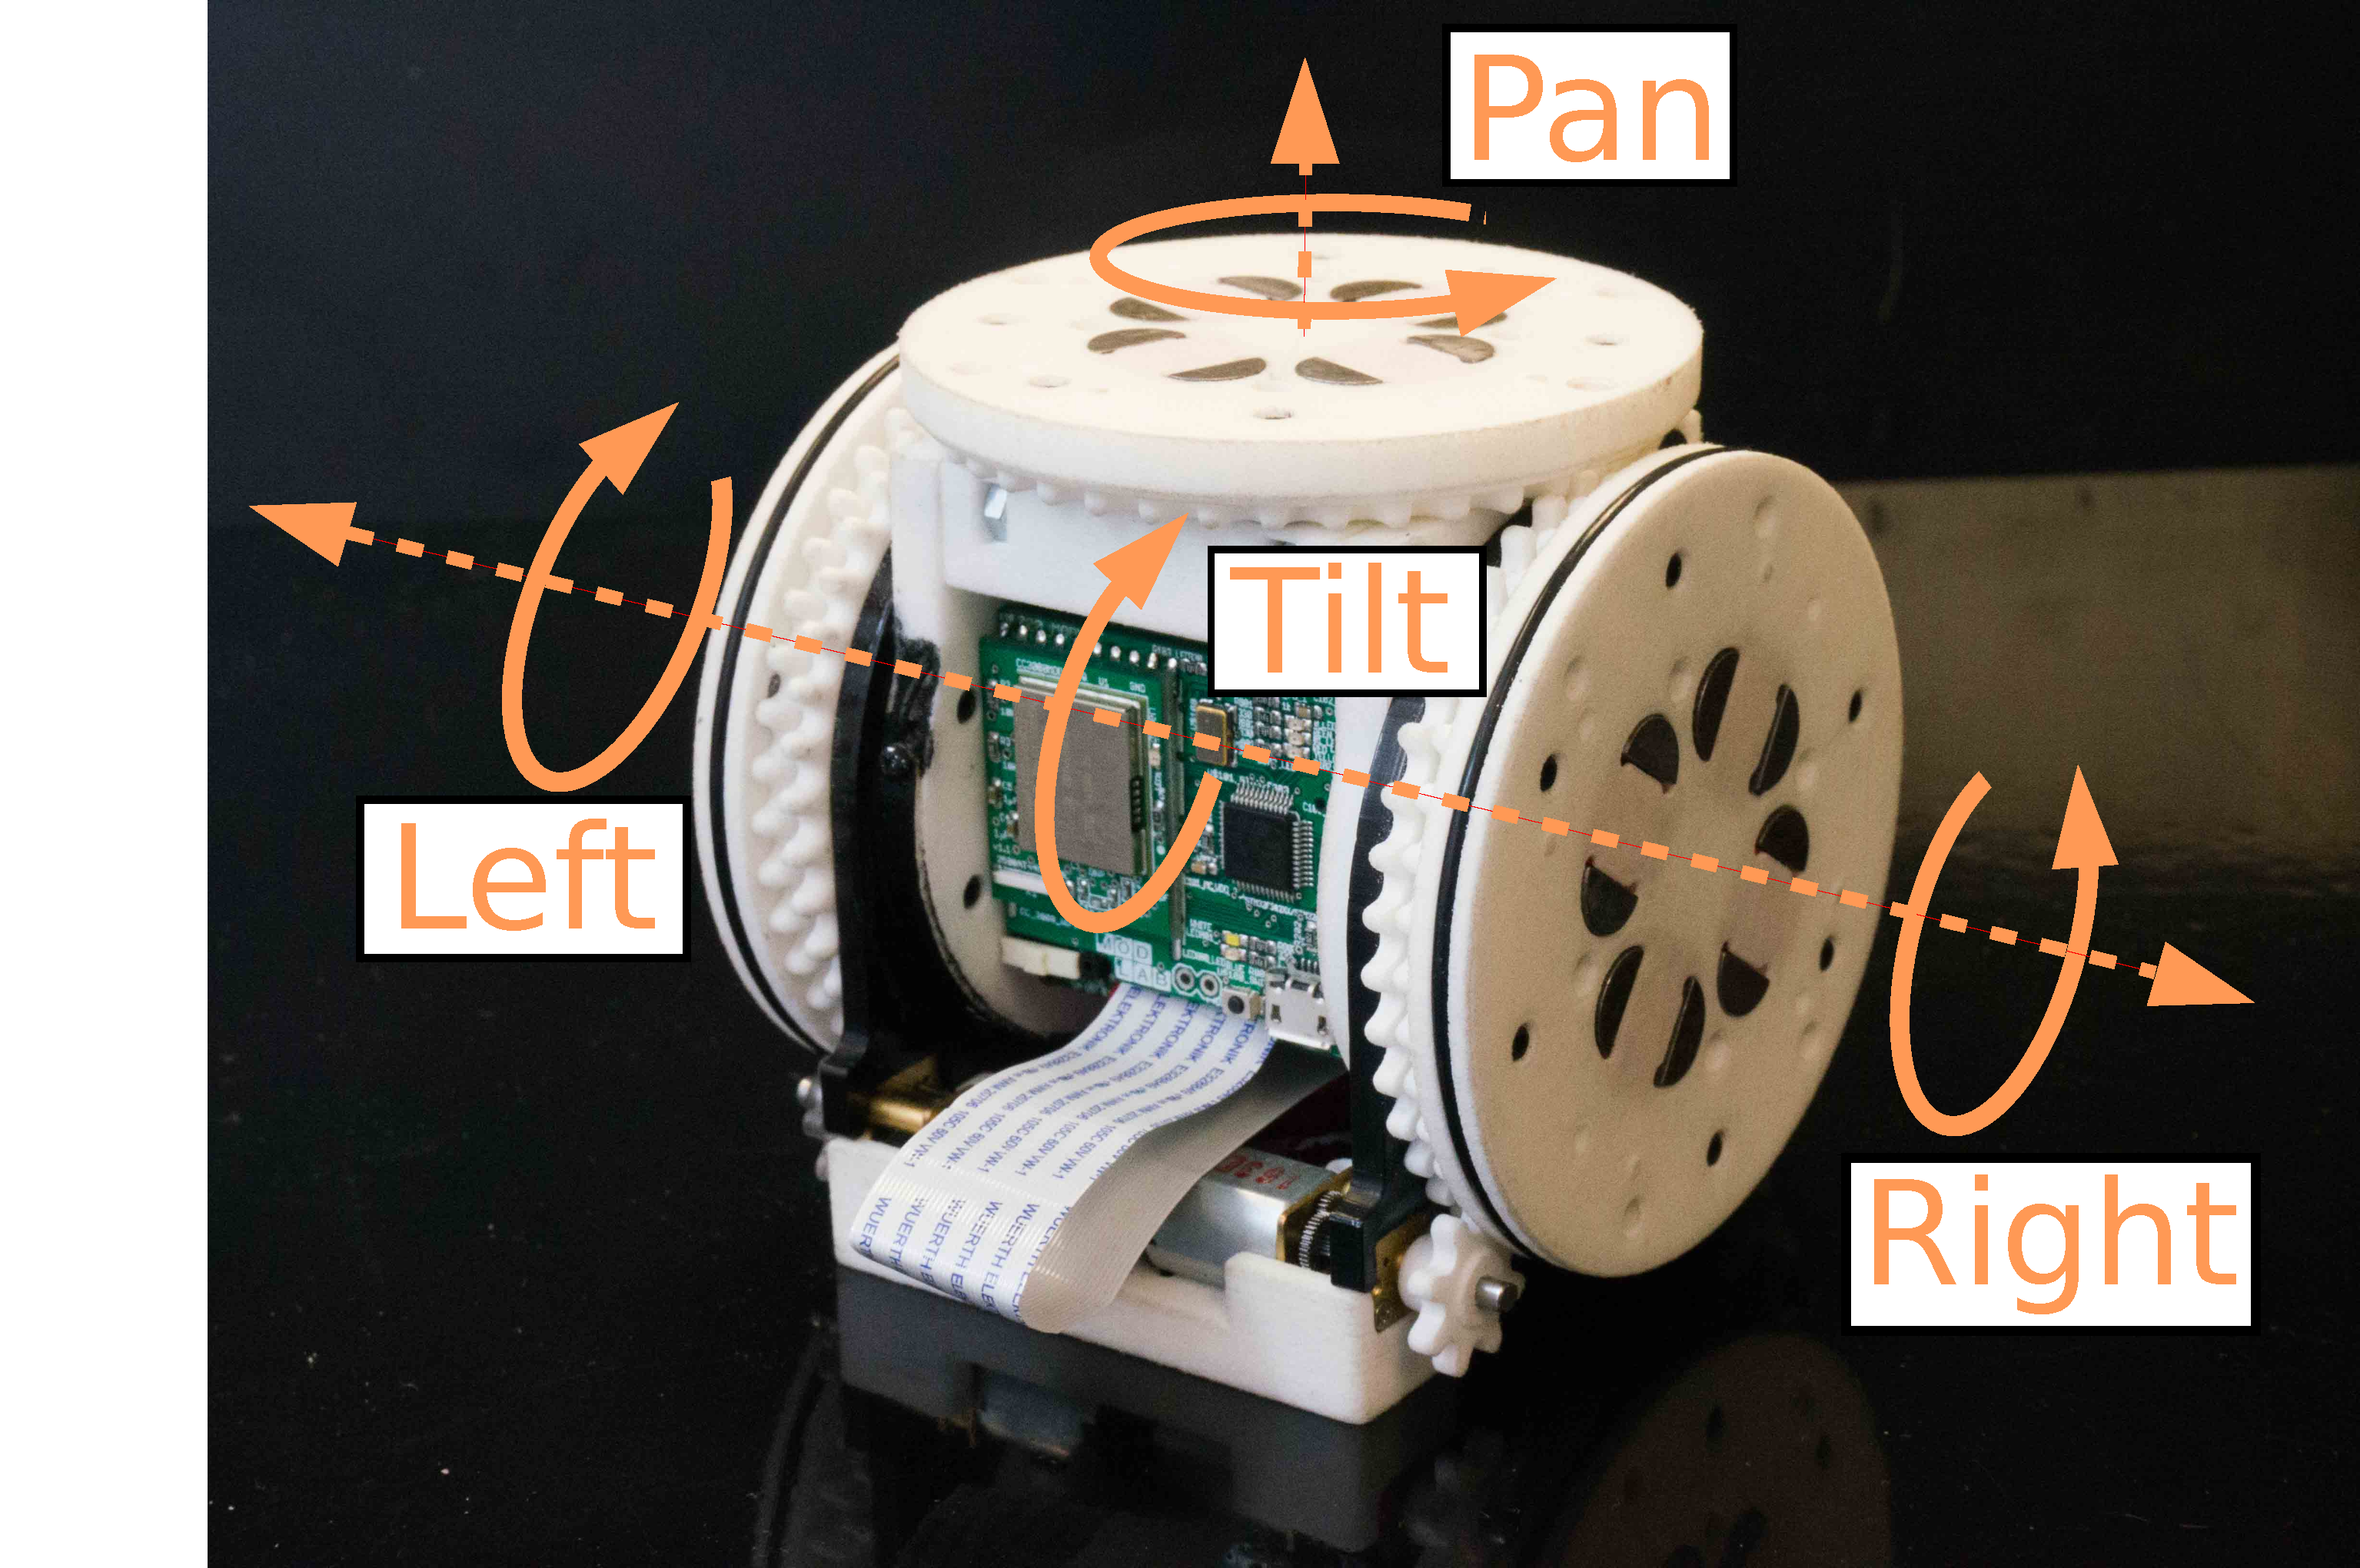
\includegraphics[height=1.5in]{images/smores_dof.pdf}
\end{center}
\caption{SMORES-EP module}
\label{fig:smores-module}
\end{figure}
%
\subsubsection{Sensor Module} % (fold)
\label{sec:sensor_module}
%
Our system architecture assumes there is a single \textit{sensor module}, containing sensors and a computer, that is carried by a cluster of modules.
%SMORES-EP modules have no sensors that allow them to gather information about their environment. To enable autonomous operation, we extend the SMORES-EP hardware by introducing a \textit{sensor module}, shown in Figure~\ref{fig:sensor-module}.
The sensor module used in our experiments was designed to work with SMORES-EP, and is shown in Figure~\ref{fig:sensor-module}.
The body of the sensor module is a 90mm $\times$ 70mm $\times$ 70mm box with thin steel plates on its front and back that allow SMORES-EP modules
to connect to it.
Computation is provided by an UP computing board with an Intel Atom 1.92 GHz
processor, 4 GB memory, and a 64 GB hard drive. A USB WiFi adapter provides
network connectivity. A front-facing Orbecc Astra Mini camera provides RGB-D
data, enabling the robot to explore and map its environment and recognize
objects of interest.  A thin stem extends 40cm above the body, supporting a
downward-facing webcam. This camera provides a view of a  0.75m $\times$ 0.5m area
in front of the sensor module, and is used to track AprilTag
\cite{olson2011apriltag} fiducials for reconfiguration. A 7.4V, 2200mAh LiPo
battery provides about one hour of running time.
%
% Sensor Module Figure
\begin{figure}
\begin{center}
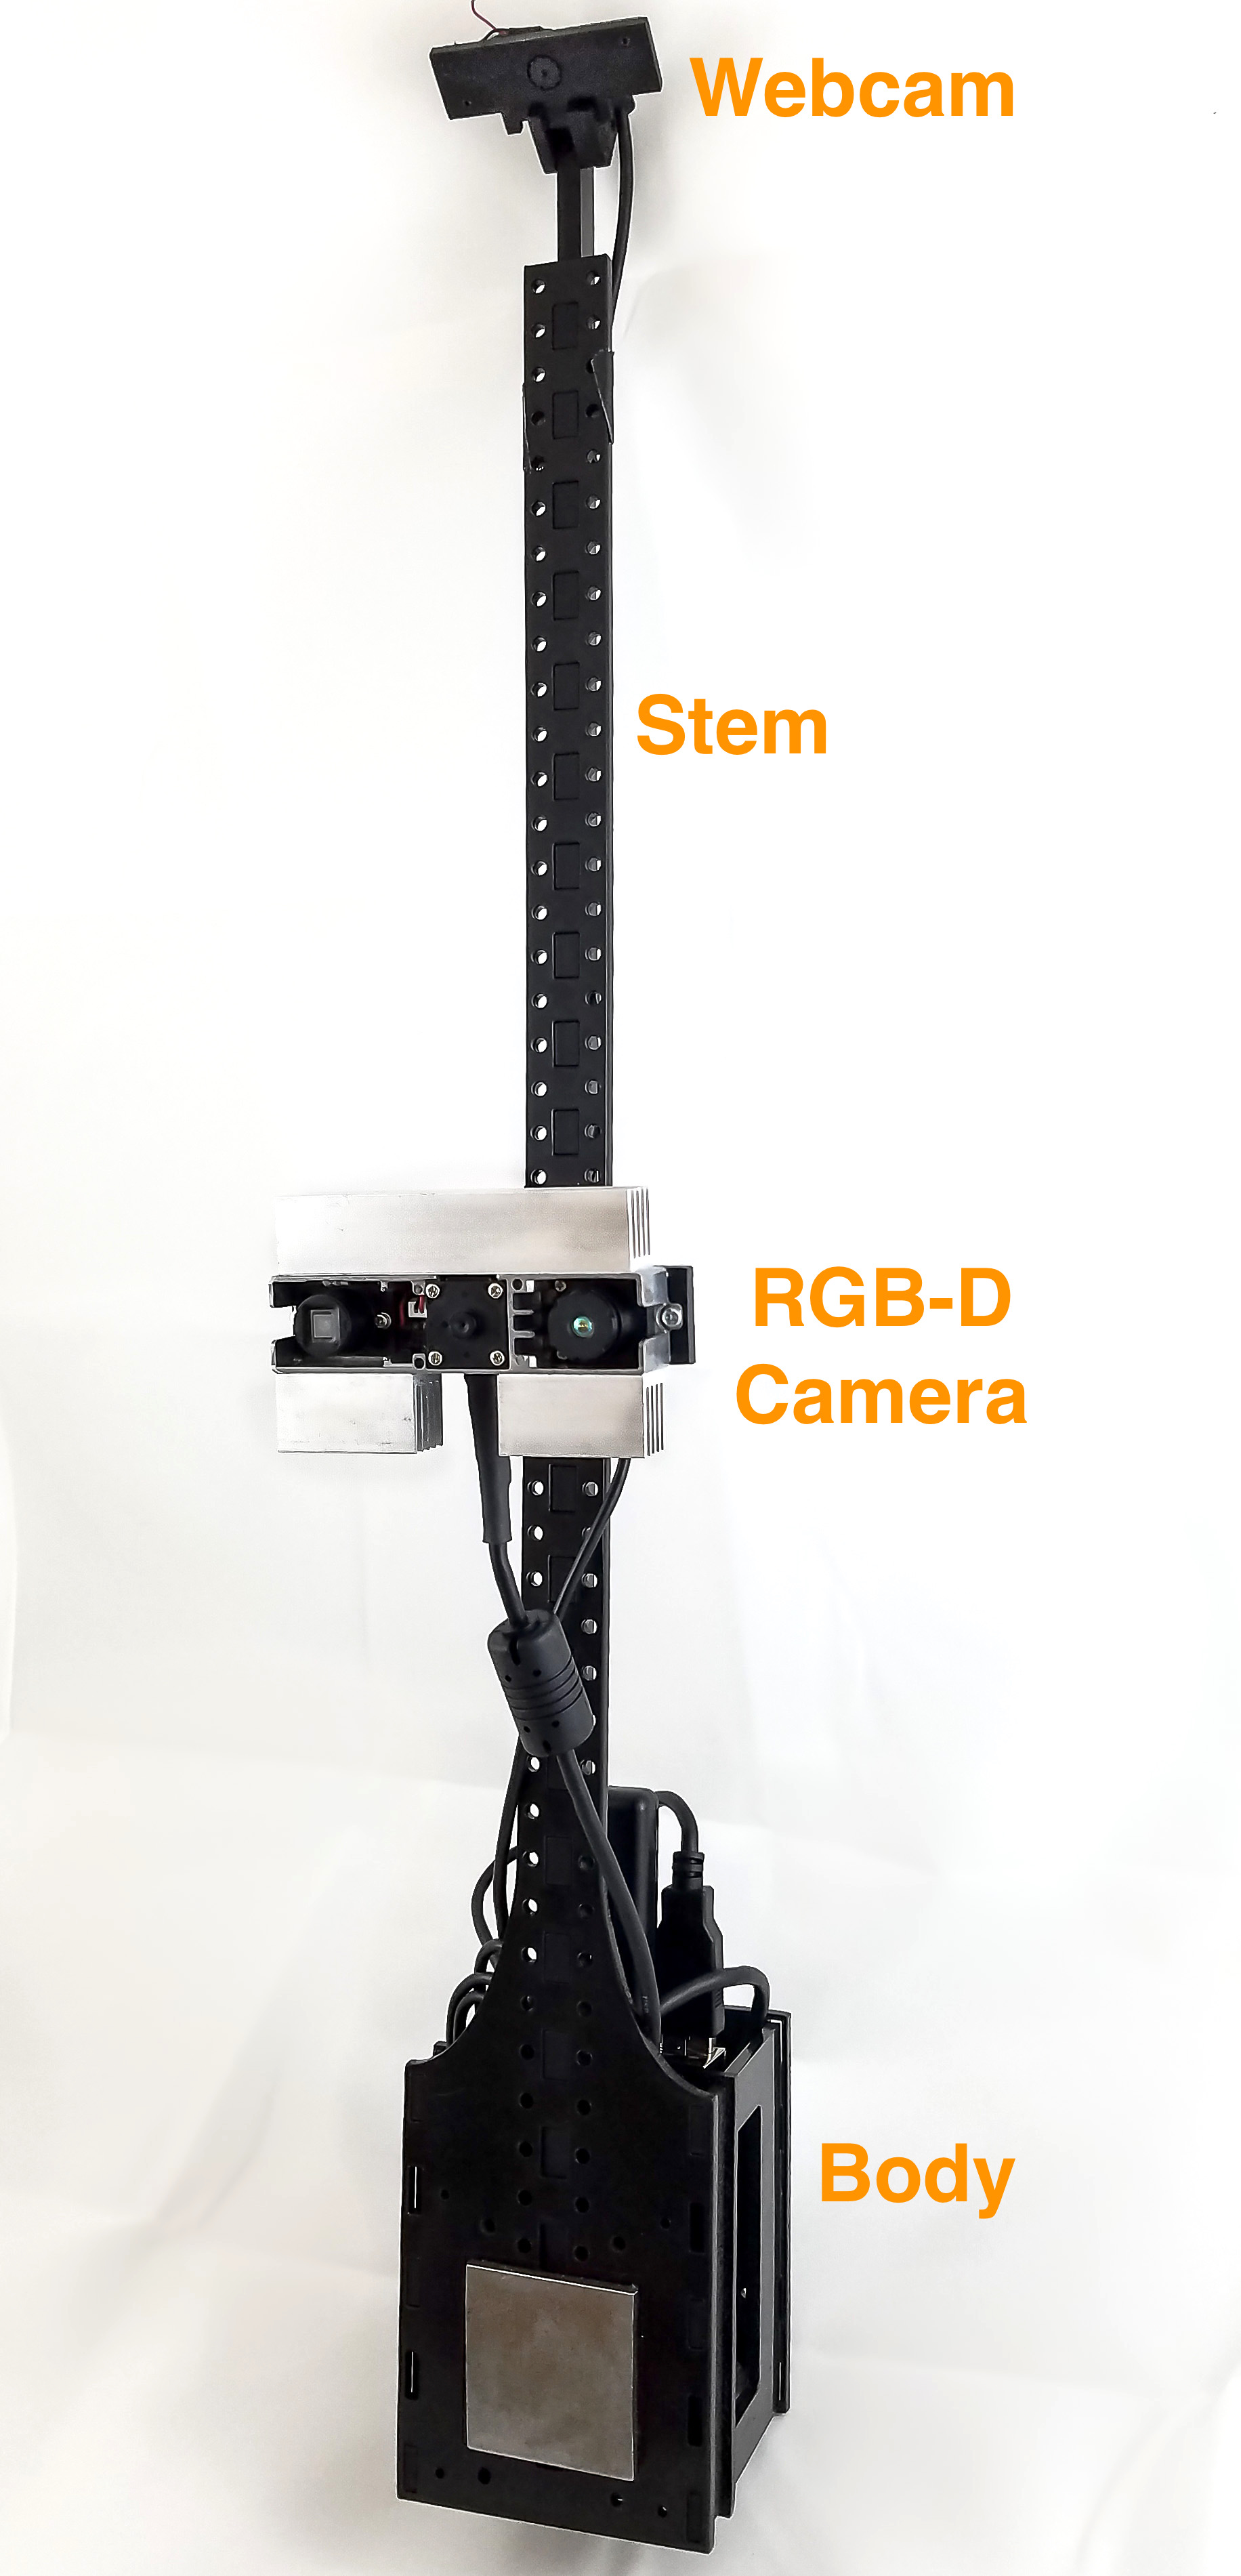
\includegraphics[width=0.3\textwidth]{images/sensor_module_new_labelled.jpg}
\caption{Sensor Module with labelled components.  UP board and battery are inside the body.}
\label{fig:sensor-module}
\end{center}
\vspace{-2em}
\end{figure}
%
%     __  ___       __          __                   __
%    / / / (_)___ _/ /_        / /   ___ _   _____  / /
%   / /_/ / / __ `/ __ \______/ /   / _ \ | / / _ \/ /
%  / __  / / /_/ / / / /_____/ /___/  __/ |/ /  __/ /
% /_/ /_/_/\__, /_/ /_/     /_____/\___/|___/\___/_/
%         /____/
%%

%     ____                            __  _
%    / __ \___  _____________  ____  / /_(_)___  ____
%   / /_/ / _ \/ ___/ ___/ _ \/ __ \/ __/ / __ \/ __ \
%  / ____/  __/ /  / /__/  __/ /_/ / /_/ / /_/ / / / /
% /_/    \___/_/   \___/\___/ .___/\__/_/\____/_/ /_/
%                          /_/
\subsection{Perception and Planning for Information}
\label{sec:exploration}
%
%Our system provides a robust suite of perception algorithms to inform control and decision-making in unknown environments.  This suite of tools serves three major functions.  First, it enables exploration, allowing the robot to map its environment, localize, and avoid obstacles.  Second, it provides the capability to recognize objects and regions of interest related to the desired task.  Third, it provides functions that characterize environment properties, providing information that allows appropriate configurations and behaviors to be selected from the design library.

%Since the proposed system performs tasks in unknown environments and conditions, a robust suite of perception algorithms is required to inform control and decision-making. The robot must have the ability to explore and build a map of its environment while avoiding obstacles and tracking its pose. The system must be able to recognize objects and regions of interest related to the desired task. Finally, the system must characterize the environment in terms of configuration capabilities. Features in the environment may restrict which robot configurations can viably perform parts of the high-level task, such as retrieving an object or navigating to a waypoint. The system needs to recognize these features to be able to intelligently choose the appropriate robot configuration for performing the task.

%The perception and exploration subsystem interprets sensor data to explore and understand the environment and inform robot behavior and adaptation. The architecture of this subsystem requires algorithms to perform SLAM, provide navigation goals for exploration, recognize objects of interest, and characterize the environment in terms of robot configuration abilities.

Completing tasks in unknown environments requires the robot to explore and gain information about its surroundings, and use that information to inform reconfiguration.
Recall in the example mail delivery task, the robot needed to explore and navigate its environment, visually locate the mailbox, and characterize the environment near the mailbox as ``stairs.''  In our system architecture, the perception and exploration subsystem is responsible for performing SLAM, providing navigation goals for exploration, and recognizing objects and regions of interest.  It is also responsible for characterizing the environment in terms of robot configurations abilities, allowing the high-level planner to make decisions regarding reconfiguration.

In our implementation, the RGB-D SLAM software package RTAB-MAP\cite{rtabmap} provides mapping and robot pose. The system incrementally builds a 3D map of the environment and stores the map in an efficient octree-based volumetric map using Octomap\cite{octomap}. The Next Best View algorithm by Daudelin et. al.\cite{Daudelin2017} enables the system to explore unknown environments by using the current volumetric map of the environment to estimate the next reachable sensor viewpoint that will observe the largest volume of undiscovered portions of objects (the Next Best View). The algorithm also estimates the amount of information (in an entropy-reduction sense) that would be gained from a sensor measurement taken at that viewpoint. The system provides the volumetric map of the environment and the reachable space of sensor viewpoints in that map to the algorithm. The algorithm then returns Next Best View waypoints to the high-level planner upon request. In the example object delivery task, the system begins the task by iteratively navigating to these Next Best View waypoints to explore objects in the environment until discovering the dropoff zone.

To identify objects of interest in the task (such as the dropoff zone), our system uses color detection and tracking.  The system recognizes colored objects using CMVision\footnote{CMVision: http://www.cs.cmu.edu/$\sim$jbruce/cmvision/}, and tracks them in 3D\footnote{Lucas Coelho Figueiredo: https://github.com/lucascoelho91/ballFollower} using depth information from the onboard RGB-D sensor. In the mail delivery example, the mailbox could be marked with a pink sign, allowing the robot to recognize it in the environment. Although we implement object recognition by color, more sophisticated methods could be included under the same system architecture.

To enable the high-level planner to choose appropriate configurations for a task, our framework requires an environment characterization algorithm. This algorithm reasons about regions of interest in the environment to classify the features in those regions of the environment. For proof-of-concept, we implemented an algorithm that can differentiate between four environment types relevant to object manipulation, shown in Figure \ref{fig:characters}. 

When the system recognizes an object in the environment, the characterization algorithm evaluates the 3D information in the object's surroundings. It creates an occupancy grid around the object location, and denotes all grid cells within a robot-radius of obstacles as unreachable (illustrated in Figure~\ref{fig:characterization}). The algorithm then selects the closest reachable point to the object within $20^o$ of the robot's line of sight to the object. If the distance from this point to the object is greater than a threshold value and the object is on the ground, the algorithm characterizes the environment as a ``tunnel''. If above the ground, it characterizes the environment as a ``stairs'' environment. If the closest reachable point is under the threshold value, the system assigns a ``free'' or ``high'' environment characterization, depending on the height of the colored object.

%In addition to characterizing the environment, the algorithm also selects a waypoint based on the characterization for the robot to position itself for reconfiguration and performing the object manipulation task. For the object delivery task, the robot characterizes the environment surrounding the dropoff zone. This enables it to determine how to reconfigure to successfully deliver the object. For example, if the environment is a ``high'' environment, it must lift the object up to be placed onto the colored zone. If the environment is a ``stairs'' environment, it must climb the stairs to drop off the object.

Based on the environment characterization and target location, the algorithm also returns a waypoint for the robot to position itself to perform its task (or to reconfigure, if necessary).  In the mail delivery example, the environment characterization algorithm directs the robot to drive to a waypoint at the base of the stairs, which is the best place for the robot to reconfigure and begin climbing the stairs.


%
% Environment types figure
\begin{figure}[t]
    \centering
    \begin{subfigure}[t]{0.15\textwidth}
        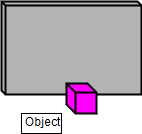
\includegraphics[width=\textwidth]{images/FreeEnvironment.png}
        %\label{fig:obja}
        \caption{\textbf{``free'}' environment}
    \end{subfigure} \ \ \ \ \ \
    \begin{subfigure}[t]{0.15\textwidth}
        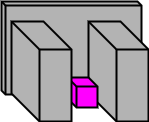
\includegraphics[width=\textwidth]{images/TunnelEnvironment.png}
        %\label{fig:objb}
        \caption{\textbf{``tunnel''} environment}
    \end{subfigure}
    
    \begin{subfigure}[t]{0.15\textwidth}
        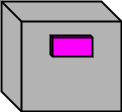
\includegraphics[width=\textwidth]{images/HighFreeEnvironment.png}
        %\label{fig:objb}
        \caption{\textbf{``high''} environment}
    \end{subfigure} \ \ \ \ \ \
    \begin{subfigure}[t]{0.15\textwidth}
        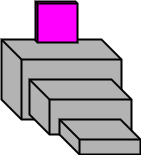
\includegraphics[width=\textwidth]{images/LedgeEnvironment.png}
        %\label{fig:objb}
        \caption{\textbf{``stairs''} environment}
    \end{subfigure}
      \caption{Environment characterization types.}
      \label{fig:characters}
\end{figure}
%
% Characterization method figure
\begin{figure}
\begin{center}
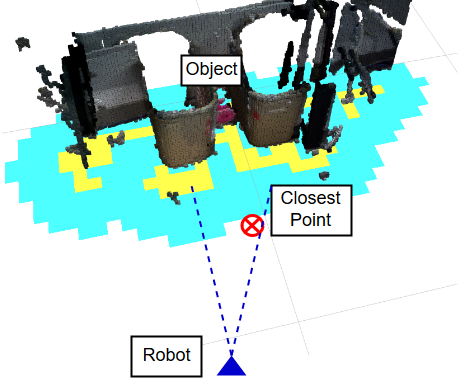
\includegraphics[width=0.4\textwidth]{images/characterization.png}
\caption{An example of a \textbf{tunnel} environment characterization. Yellow grid cells are occupied, light blue cells are unreachable resulting from bloating obstacles.}
\label{fig:characterization}
\end{center}
\vspace{-2em}
\end{figure}

%    ______            _____          _____                 _ _____
%   / ____/___  ____  / __(_)___ _   / ___/____  ___  _____(_) __(_)_________
%  / /   / __ \/ __ \/ /_/ / __ `/   \__ \/ __ \/ _ \/ ___/ / /_/ / ___/ ___/
% / /___/ /_/ / / / / __/ / /_/ /   ___/ / /_/ /  __/ /__/ / __/ / /__(__  )
% \____/\____/_/ /_/_/ /_/\__, /   /____/ .___/\___/\___/_/_/ /_/\___/____/
%                        /____/        /_/
\subsection{Library of Configurations and Behaviors}
\label{sec:configuration-specifics}
%
In this work, we use the architecture introduced in \cite{Jing2016}. We encode the full set of capabilities of the modular robot, such as driving and picking up items, in a library of robot configurations and behaviors.
Specifically, we label each entry with attributes that describe what it does, as well as the environment conditions under which it may be used. 
This allows the high-level planner to match environment characterizations from the perception subsystem with configurations and behaviors that can perform the task in the current environment. 
In the case of our mail delivery example, when the environment characterization algorithm reports that the mailbox is located in a ``stairs''-type environment, the high-level planner queries the library for configurations that can climb stairs.  
Since the library indicates that current configuration is only capable of driving on flat ground, the high-level planner opts to reconfigure to the stair-climber configuration, and executes its \textbf{climbUp} behavior.

Our implementation relies on a framework first presented in \cite{Jing2016}, which we summarize here.
In this framework, a library entry is defined as $l = (C,B_C,P_b,T_e)$ where:
\begin{itemize}
\item $C$ is the robot \emph{configuration}, specified by the connected structure of the modules.
\item $B_C$ is a \emph{behavior} that $C$ can perform. A behavior is a controller that specifies commands for robot joints to perform a specific action. 
\item $P_b$ is a set of \emph{behavior properties} that describes what $B_C$ does. 
\item $T_e$ is a set of \emph{environment types} that describe the environments in which this library entry is suitable. 
\end{itemize} 
%
When we specify tasks at the high level, we use behavior properties $P_b$ to describe a desired robot action without explicitly specifying a configuration or behavior.
Environment types $T_e$ specify the conditions under which a behavior can be used.
%, and are determined through the environment characterization processes described in Section~\ref{sec:exploration}.

To create robot configurations and behaviors, we utilize the VSPARC (Verification, Simulation, Programming And Robot Construction \footnote{\url{www.vsparc.org}}) simulator presented in \cite{Jing2016}.
VSPARC allows users to design, simulate and test configurations and behaviors for the SMORES-EP robot system.
Our system can then use the behavior designs to control the physical SMORES-EP robot to perform various actions.

In \cite{Jing2016}, all robot behaviors are \textit{static} behaviors.
That is, once users create a behavior in VSPARC, joint values for each module are fixed and cannot be modified during behavior execution.
Static behaviors, such as a car with a fixed turning radius, do not provide enough maneuverability for the robot to navigate around unknown environment.
In this work, we expand the type of behaviors in the library by using \textit{parametric} behaviors, which were first introduced in \cite{JingAURO2017}.
Parametric behaviors have joint commands that can be altered during run-time, and therefore allow a wider range of motions.
For example, a parametric behavior for a car configuration can be a driving action with two parameters: turning angle and driving velocity.  
The system associates a parametric behavior with a program that generates values of joint commands based on environment information and current robot tasks.
Recall the mail delivery task, based on the sensed environment, the perception and exploration subsystem (Section~\ref{sec:exploration}) can generate a collision-free path, which is used to calculate real-time velocity for the robot to follow the path.
Our system then converts the robot velocity to joint values in parametric behaviors during run-time.

The library introduced in \cite{Jing2016} has 57 robot configurations and 97 behaviors.
Here we list 10 entries for four different configurations in Table~\ref{table:1} that are used in this work.
%This library was created to enables the robot to explore and interact with the environment and objects, but the library can be expanded to include more entries for other environments and tasks. 
Note that each library entry consists of a configuration with its available behaviors subject to restrictions in environment conditions. To characterize the environment in terms of these restrictions, we use the perception algorithm described in Section \ref{sec:exploration}.

To provide an illustrative example, we discuss two configurations and their capabilities in detail.
The ``Car'' configuration shown in Figure~\ref{fig:dropoff} is capable of picking
up and dropping objects in a ``free'' environment. In addition, the ``Car'' configuration can locomote on flat terrain. It uses a parametric differential drive behavior to convert a desired velocity vector into motor commands (\textbf{drive} in Table \ref{table:1}).

The ``Proboscis'' configuration shown in Figure~\ref{fig:pink_grab} has
a long arm in front, and is suitable for reaching between obstacles in a narrow ``tunnel'' environment to grasp objects or reaching up in a ``high'' environment to drop items.
However, the locomotion ability of this configuration is limited to forward/backward
motion, making it unsuitable for general navigation.

This library-based framework allows users to express desired robot actions in an abstract way by specifying behavior properties. For example, if a task specifies that the robot should execute a behavior with the \textbf{drop} property, our system could choose to use either the Car or Proboscis configurations to perform the action, since both have behaviors with the \textbf{drop} property.
The decision of which configuration to use is made during task execution, based on the sensed environment.
For example, if the perception system reports that the environment is of type ``tunnel'', the Proboscis configuration will be used, because the library indicates that it can be used in ``tunnel''-type environments while the Car cannot.

% I moved the disccusion about this to highlevel %Since self-reconfiguration is time-consuming, decisions are biased toward behaviors associated with the current configuration whenever possible, so that the robot only reconfigures when it is necessary to complete a task.
%
\begin{table}
\centering
\begin{tabular}{ |c|c|c| } 
 \hline
 \multirow{2}{6em}{Configuration} & Behavior & Environment \\
 & properties & Types \\
 \hline
 \multirow{3}{*}{Car} & \textbf{pickUp} & ``free'' \\\cline{2-3}
  & \textbf{drop} & ``free'' \\\cline{2-3}
  & \textbf{drive} & ``free''\\ \hline
 \multirow{3}{*}{Proboscis} & \textbf{pickUp} & ``tunnel'' or ``free''\\ \cline{2-3}
  & \textbf{drop} &``tunnel'' or ``free'' \\ \cline{2-3}
  & \textbf{highReach} & ``high''\\ \hline
 Scorpion & \textbf{drive} & ``free''\\ \hline
 \multirow{3}{*}{Snake} & \textbf{climbUp} & ``stairs''\\ \cline{2-3}
  & \textbf{climbDown} & ``stairs''\\ \cline{2-3}
  & \textbf{drop} & ``stairs'' or ``free''\\
 \hline
\end{tabular}
\caption{A library of robot behaviors}
\label{table:1}
\vspace{-1em}
\end{table}

%     ____                        _____                        __  _
%    / __ \___  _________  ____  / __(_)___ ___  ___________ _/ /_(_)___  ____
%   / /_/ / _ \/ ___/ __ \/ __ \/ /_/ / __ `/ / / / ___/ __ `/ __/ / __ \/ __ \
%  / _, _/  __/ /__/ /_/ / / / / __/ / /_/ / /_/ / /  / /_/ / /_/ / /_/ / / / /
% /_/ |_|\___/\___/\____/_/ /_/_/ /_/\__, /\__,_/_/   \__,_/\__/_/\____/_/ /_/
%                                   /____/
\subsection{Reconfiguration}
\label{sec:reconfiguration}
%
When the high-level planner decides to use a new configuration during a task, the robot must reconfigure. Our system architecture allows any method for reconfiguration, provided that it requires no external sensing. SMORES-EP is capable of all three classes of modular self-reconfiguration (chain, lattice, and mobile reconfiguration) \cite{Davey2012,yim2003modular}.  We have implemented tools for mobile reconfiguration with SMORES-EP, taking advantage of the fact that individual modules can drive on flat surfaces as described in Section \ref{sec:hardware}.

Determining the relative positions of modules during mobile self-reconfiguration is an important challenge. 
%As discussed in Section~\ref{sec:related-work}, past systems have relied on offboard global positioning systems \cite{Paulos2015} or distributed approaches, in which sensors are mounted on each disconnected set of modules \cite{Yim2007}.  
Our localization method is centralized, using a camera carried by the robot to track AprilTag fiducials mounted to individual modules.
As discussed in Section~\ref{sec:hardware}, the camera provides a view of a $0.75\text{m}\times0.5\text{m}$ area on the ground in front of the sensor module.  
Within this area, our system provides pose for any module equipped with an AprilTag marker to perform reconfiguration. 
%Within this area (which we call the \emph{reconfiguration zone}), any module equipped with an AprilTag marker can detach from the cluster, drive to another location, and reattach to the cluster, provided that both of its wheels were in contact with the ground in its starting position.% \TODO{Get accurate number for height and FoV.}

%\subsection{Reconfiguration Procedure}
Given an initial configuration and a goal configuration, our reconfiguration controller commands a set of modules to disconnect, move and reconnect in order to form the new topology of the goal configuration. 
The robot first takes actions to establish the conditions needed for reconfiguration. 
It begins by confirming that the reconfiguration zone is a flat surface free of obstacles (other than the modules themselves).
%If the robot is carrying an object, it drops the object outside of the reconfiguration zone.
It then sets its joint angles so that all modules that need to detach have both of their wheels on the ground, ready to drive.
Then the robot performs operations to change the topology of the cluster by detaching a module from the cluster, driving, and re-attaching at its new location in the goal configuration, as shown in Figure~\ref{fig:reconf}.
Currently, reconfiguration plans from one configuration to another are created manually and stored in the library.  In the future, existing assembly planning algorithms (\cite{Werfel2007,Seo2013}) could be adapted to generate reconfiguration plans automatically.
Because the reconfiguration zone is free of obstacles, we compute collision-free paths offline and store them as part of the reconfiguration plan.
Once all module movement operations have completed and the goal topology is formed, the robot sets its joints to appropriate angles for the goal configuration to begin performing desired behaviors.
%, and if necessary, the robot picks up any objects it dropped. This completes the reconfiguration process.

%The process consists of three stages: i) Pre-reconfiguration, ii) Module Movement, iii) Post-reconfiguration.

%\paragraph{Pre-reconfiguration} In the pre-reconfiguration stage, the robot takes actions to establish the conditions needed for reconfiguration.  It begins by confirming that the reconfiguration zone is a flat surface free of obstacles (other than the modules themselves).  If the robot is carrying an object, it drops the object outside of the reconfiguration zone. It then  sets its joint angles so that all modules that need to detach have both of their wheels on the ground, ready to drive. Once these conditions are established, module movement begins.

%\paragraph{Module Movement} During this stage, the topology of the cluster changes as a sequence of module movement operations are performed.  Each operation changes the topology of the cluster by detaching a module from the cluster, driving, and re-attaching at its new location in the goal configuration, as shown in Figure~\ref{fig:reconf}.

%In order to transform from an initial configuration to a goal configuration, a feasible reconfiguration plan (sequence of module movement operations) must be supplied before reconfiguration begins.  Each configuration in the library has an associated set of reconfiguration plans that allows it to transform to other configurations in the library.  Currently, reconfiguration plans are created by hand.  In the future, existing assembly planning algorithms (\cite{Werfel2007,Seo2013}) could be adapted to generate reconfiguration plans automatically.

% We denote a module movement operation as $MP=\left(m, m_d, m_a, f_m^d, f_m^a, f_{m_d}, f_{m_a}, \sigma \right)$ where:
% \begin{itemize}
% \item $m$ is the module whose location will be changed in this module operation.
% \item $m_d$ is the module that connects with $m$ before the operation.
% \item $m_a$ is the module that connects with $m$ after the operation. Notice $m_d$ and $m_a$ can be the same module. 
% \item The face $f_m^d$ of module $m$ connects with the face $f_{m_d}$ of module $m_d$ before the operation.
% \item The face $f_m^a$ of module $m$ connects with the face $f_{m_a}$ of module $m_a$ after the operation. Notice $f_m^d$ and $f_m^a$ can be the same face. In this work, we assume $f_m^a$ can only be the front or the back face of the module $m$.
% \item $\sigma$ is the path that module $m$ will follow during the operation.
% \end{itemize}

%To travel from its initial location to its final location, a module uses its left and right wheels to move by differential-drive.  Because the reconfiguration zone is free of obstacles, collision-free paths can be pre-computed and stored as part of the reconfiguration plan.  Paths can also be computed at runtime if desired.  AprilTag localization allows the robot to follow the path.

We developed several techniques to ensure reliable connection and disconnection during reconfiguration.  
When a module disconnects from the cluster, the electro-permanent magnets on the connected faces are turned off.  To guarantee a clean break of the magnetic connection, the disconnecting module bends its tilt joint up and down, mechanically separating itself from the cluster. During docking, accurate alignment is crucial to the strength of the magnetic connection \cite{tosun2016design}.  For this reason, rather than driving directly to its final docking location, a module instead drives to a pre-docking waypoint directly in front of its docking location.  At the waypoint, the module spins in place slowly until its heading is aligned with the dock point, and then drives in straight to attach. To guarantee a good connection, the module intentionally overdrives its dock point, pushing itself into the cluster while firing its magnets.
%
\begin{figure}[t]
\begin{center}
  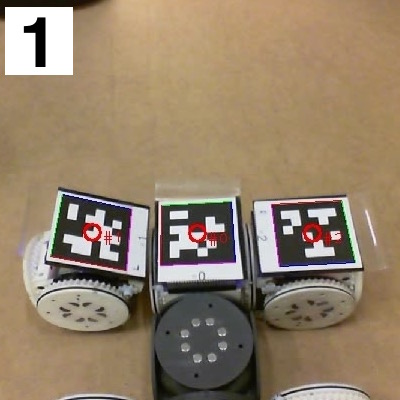
\includegraphics[width=0.32\columnwidth]{images/reconf_detach.jpg}
  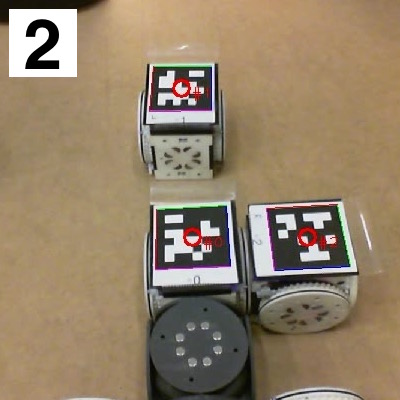
\includegraphics[width=0.32\columnwidth]{images/reconf_waypoint.jpg}
  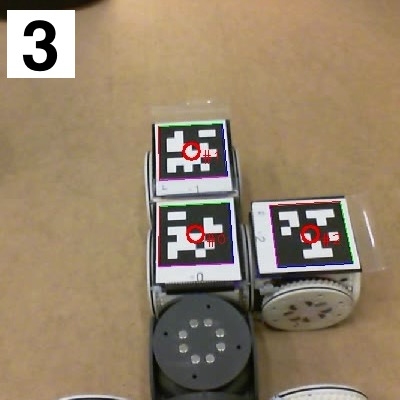
\includegraphics[width=0.32\columnwidth]{images/reconf_attach.jpg}
  \caption{Module movement during reconfiguration. (1) Left module detaches from cluster. (2) Module drives to waypoint, and spins to establish its heading. (3) Module drives straight in to dock point, and reattaches.}
  \label{fig:reconf}
\end{center}
\end{figure}

%\paragraph{Post-reconfiguration} Once all module movement operations have completed and the goal topology is formed, the robot sets its joints to appropriate angles for the goal configuration to begin performing desired behaviors, and if necessary, the robot picks up any objects it dropped. This completes the reconfiguration process. 

\subsection{High-Level Planner}
\label{sec:high-level}
In our architecture, the high-level planner subsystem provides a framework for users to specify tasks  at a high level using a formal language, and acts as the main, centralized controller that directs robot motion and actions based on the given tasks.  Users do not specify the configurations and behaviors used to complete tasks, but rather describe desired actions in terms of goals and outcomes.  Returning to our mail delivery example, the user indicates that the robot should \textbf{explore} until it locates the \textbf{mailBox}, then \textbf{drop} the object off.  The sequence of configurations and behaviors used to complete this task is not specified by the user, but instead determined by the high-level planner as it continually reacts to the sensed environment.

The high-level planner coordinates each component introduced in previous sections to form a system for controlling our MSRR to achieve complex tasks.
At system level, the sensing components gather and process environment information for the high-level planner, which then takes actions based on the given robot tasks by invoking appropriate low-level behaviors.

We abstract the robot and environment status as a set of Boolean propositions.
In the mailbox example, the robot action \textbf{drop} is \lt if the robot is currently dropping an object to the mailbox (and \lf otherwise) and the environment proposition \textbf{mailBox} is \lt if the robot is currently sensing a mailbox (and \lf otherwise).
Moreover the proposition \textbf{explore} encodes whether or not the robot is currently searching for the target, the mailbox in this case.
%A wide range of reactive robotic tasks can be specified in terms of these propositions.
By using a library of robot configurations and behaviors as well as environment characterization tools, we can map these high-level abstraction to low-level sensing programs and robot controllers.
%To see how this works, consider Specification~\ref{spec:experiment}, which shows  high-level instructions from the user that direct the robot to explore a room, search, and move any object of interest to a drop-off zone.
As discussed in Section~\ref{sec:configuration-specifics}, the user specifies high-level robot actions in terms of behavior properties from the library. 
In the mail delivery example, our system can choose to do a drop action by executing any behavior from the library which has the behavior property \textbf{drop}, and which also satisfies the current ``stairs''-type environment. If the current robot configuration cannot execute an appropriate behavior, the robot will reconfigure to a different configuration that can.  In this way, the system autonomously chooses to implement  \textbf{drop}  appropriately in response to the sensed environment.
Our system evaluate propositions related to the state of the environment using perception and environment characterization tools in Section~\ref{sec:exploration}. For example, we can map proposition \textbf{mailBox} to the color tracking function in our perception subsystem, which assign the value \lt to \textbf{mailBox} if and only if the robot is currently seeing a mailbox with the onboard camera.
The system treats propositions, such as \textbf{explore}, that require the robot to navigate in the workspace differently from the other simple robot actions, such as \textbf{drop}.
In this example, we can map \textbf{explore} to behavior property \textbf{drive}, which represents a set of parametric behaviors as discussed in Section~\ref{sec:configuration-specifics}.
In order to obtain joint values for behaviors at run-time, a path planner in the perception and planning subsystem (Section~\ref{sec:exploration} takes into account the robot goal as well as the current environment information from  our perception subsystem, and generates a collision-free path for the robot to follow.
Our system then converts this path to joint values, which are used to execute the \textbf{drive} behaviors.
%in Specification~\ref{spec:experiment}, the proposition \textbf{arrived} is \lt if the robot arrives at its target location, which is determined by consulting the robot's position in the map generated by SLAM. The proposition \textbf{dropoffZone} is \lt if the robot is currently sensing a drop-off zone, which is determined by consulting both the map and color tracking functions.

%The user specifies high-level robot actions in terms of behavior properties from the library.  For example, Line 7 in Specification~\ref{spec:experiment} specifies that under certain conditions, the robot should do \textbf{pickUp}.  As discussed in Section~\ref{sec:configuration-specifics}, our system can choose to do \textbf{pickUp} by executing any behavior from the library which has the behavior property \textbf{pickUp}, and which also satisfies the current environment characteristics. If the current robot configuration cannot execute an appropriate behavior, the robot will reconfigure to a different configuration that can.  In this way, the system autonomously chooses to implement  \textbf{pickUp}  appropriately in response to the sensed environment.

%Some robot actions, such as \textbf{driveExplore}, \textbf{driveToObject}, and \textbf{driveToDropoff}, requires the robot to navigate in the environment without colliding with obstacles.
%To achieve this, a goal pose is first determined by the controller and sent to a path planning program to generate a collision free path while considering the dynamics of the robot.
%The path is then converted to a sequence of robot velocity vectors and used as the input to control a parametric driving behavior in the library.
%In this work, we use the ROS navigation package\footnote{http://wiki.ros.org/navigation} to generate paths for a differential drive robot to control the ``Car'' configuration in the library.

%Propositions related to the state of the environment are evaluated using the perception tools described in Section~\ref{sec:exploration}. For example in Specification~\ref{spec:experiment}, the proposition \textbf{arrived} is \lt if the robot arrives at its target location, which is determined by consulting the robot's position in the map generated by SLAM. The proposition \textbf{dropoffZone} is \lt if the robot is currently sensing a drop-off zone, which is determined by consulting both the map and color tracking functions.

%\begin{spec}[h!]
%\caption{Search and move any object of interest to the drop-off zone}
%\label{spec:experiment}
%\vspace{-0.1cm}
%\small\setlength{\jot}{0pt}
%\begin{fleqn}[3pt]
%\leqnomode
%\begin{subequations}
%\renewcommand{\theequation}{\arabic{equation}} 
%\makeatletter
%\renewcommand\tagform@[1]{\maketag@@@{\ignorespaces#1\unskip\@@italiccorr}}
%\makeatother
%\hskip-10cm
%\begin{alignat}{2}
%&\text{{\bf 1.} {\bf carry} is set on {\bf pickUp} and reset on {\bf drop}}&& \notag \\
%&\text{{\bf 2.} if you are not activating ({\bf pickUp} or {\bf drop} or {\bf driveToObject}}&& \notag \\
%&\hspace{1cm}\text{or {\bf driveToDropoff} or {\bf carry}) then do {\bf driveExplore}}&& \notag \\
%&\text{{\bf 3.} if you are activating {\bf carry} and you are not sensing }&& \notag \\
%&\hspace{1cm}\text{{\bf dropoffZone} then do {\bf driveExplore}}&& \notag \\
%&\text{{\bf 4.} do {\bf driveToDropoff} if and only if you are activating {\bf carry} }&& \notag \\
%&\hspace{1cm}\text{and you are sensing {\bf dropoffZone}}&& \notag \\
%&\text{{\bf 5.} do {\bf driveToObject} if and only if you are not activating {\bf carry} }&& \notag \\
%&\hspace{1cm}\text{and you are sensing {\bf object}}&& \notag \\
%&\text{{\bf 6.} do {\bf drop} if and only if you were activating {\bf driveToDropoff } }&& \notag \\
%&\hspace{1cm}\text{and you are sensing {\bf arrived}}&& \notag \\
%&\text{{\bf 7.} do {\bf pickUp } if and only if you were activating {\bf driveToObject} }&& \notag \\
%&\hspace{1cm}\text{and you are sensing {\bf arrived}}&& \notag \\
%&\text{{\bf 8.} infinitely often not {\bf carry}}&& \notag
%\end{alignat}
%\end{subequations}
%\end{fleqn}
%\vspace{-0.4cm}
%\end{spec}


Our implementation employs an existing tool called LTLMoP (Linear Temporal Logic MissiOn Planning) to automatically generate robot controllers from user-specified high-level instructions using logic synthesis \cite{DBLP:conf/iros/FinucaneJK10,DBLP:journals/trob/Kress-GazitFP09}.
The user describes the desired robot tasks with high-level specification over the set of abstracted robot and environment propositions that are mapped to behavior properties from the library.
LTLMoP automatically converts the specification to logic formulas, which are then used to synthesize a robot controller that satisfies the given tasks (if one exists).
The controller is in the form of a finite state automaton, as shown in Figure~\ref{fig:autSimple}.
Each state specifies a set of high-level robot actions that need to be performed, and transitions between states include a set of environment propositions.
Note some of propositions are omitted in Figure~\ref{fig:autSimple} for clarity.
Execution of the high-level controller begins at the predefined initial state in the finite state automaton. In each iteration, LTLMoP determines the values of all environment propositions by calling the corresponding sensing program. Then, LTLMoP chooses the next state in the finite state machine by taking the transition that matches the current value of all environment propositions. 
In the next state, for each robot proposition LTLMoP chooses a behavior from the design library which satisfies both the behavior properties and current environment type.
For example, in Figure~\ref{fig:autSimple} we start in the top state and execute the \textbf{explore} program.
If  the robot senses a mailbox, the value of \textbf{mailBox} is \lt and therefore the next state is the bottom right state. We then stop the \textbf{explore} program and execute the \textbf{driveToMailBox} program.
Since self-reconfiguration is time-consuming, the controller chooses to execute the selected behavior using the current robot configuration whenever possible.
If the current configuration cannot execute the behavior, the controller instructs the robot to reconfigure to one that can, and if multiple appropriate configurations are available, the controller selects one at random.

\begin{figure}
\begin{center}
\includegraphics[width=0.4\textwidth]{images/autSimple.png}
\caption{An example of a synthesized controller automaton. A proposition with ``!'' has a value of \lf, and \lt otherwise.}
\label{fig:autSimple}
\end{center}
\end{figure}

%Since the synthesized high-level controller is a discrete finite state automaton, we need to implement it continuously in order to control the robot to satisfy the given task.
%Execution of the high-level controller begins at the predefined initial state in the finite state automaton. In each iteration, the values of all environment propositions are determined by calling the corresponding sensing program. Then, we determine the next state in the finite state machine by taking the transition that matches the current value of all environment propositions. 
%In the next state, the specified high level behavior properties are mapped to a behavior from the design library which satisfies both the behavior properties and current environment type.
%The system then maps the system proposition specified in the next state to its set of behavior properties, and selects a behavior from the design library which satisfies both the behavior properties and current environment properties.
%If the robot is not currently in a configuration capable of executing the selected behavior, the system commands the robot to reconfigure. Finally, the behavior is executed, and the program continues on to the next iteration. 




%     ______                     _                      __
%    / ____/  ______  ___  _____(_)___ ___  ___  ____  / /______
%   / __/ | |/_/ __ \/ _ \/ ___/ / __ `__ \/ _ \/ __ \/ __/ ___/
%  / /____>  </ /_/ /  __/ /  / / / / / / /  __/ / / / /_(__  )
% /_____/_/|_/ .___/\___/_/  /_/_/ /_/ /_/\___/_/ /_/\__/____/
%           /_/
\section{Experiment Results}
\label{sec:experiments}
%

In three hardware experiments, we demonstrate how our system allows the robot to autonomously explore, decide how and when to reconfigure, and manipulate objects to complete tasks in unknown environments. Table \ref{table:task-compare} presents the environments and tasks in each experiment.
In Experiment I, the robot completes a complex, multi-part object retrieval task that requires significant exploration, reactive decision-making, and reconfiguration in response to its environment.
Experiments II and III give the robot the task of delivering an object to an \textit{a priori} unknown goal) in two different environments.  The system reacts to the two scenarios by taking very different actions, both requiring reconfiguration.

These experiments accomplish two goals.  First, they fill an experimental
gap in the field, representing the first evidence of a modular robot autonomously reconfiguring in response to its perceived (\textit{a priori} unknown) environment in order to complete tasks.  Second, they provide observations and insights into the challenges presented by autonomous modular robot systems.  By discussing lessons learned, others may build on our work and create even more capable systems. 

%As mentioned earlier, our work presents the first MSRR system that uses perception and reconfiguration to autonomously perform high-level tasks in unknown environments. We tested our system implementation on multiple, real-world tasks.
%These experiments accomplish two goals: First, they demonstrate our system's ability to autonomously adapt to multiple unknown environments and to complete different tasks. 
%Second, they provide new observations of challenges with fully autonomous MSRR systems. These observations provide insight on what can be improved in autonomous MSRR systems to make them more robust and versatile.

%Three experiments were run, each time varying the environment and the type of task to be performed. Each experiment required the robot to explore an unknown environment to search for and identify one or more objects of interest, and then complete some manipulation task with those objects.

\newcommand{\Lwidth}{0.5\columnwidth}
\newcommand{\Rwidth}{0.4\columnwidth}
%\newcommand{\Tbuffer}{-2cm}
\newcommand{\Rboxheight}{-0.5\height}
\setlength{\tabcolsep}{4pt} %reduces horizontal padding in table. 
%\renewcommand{\arraystretch}{5}
\begin{table}
\centering
\begin{tabular}{|c|c|}
\hline
 & \vspace{-5pt}\\

\textbf{Environment Setup} & \textbf{Task Description}\\

\hline
 & \vspace{-5pt}\\
 
\raisebox{\Rboxheight}{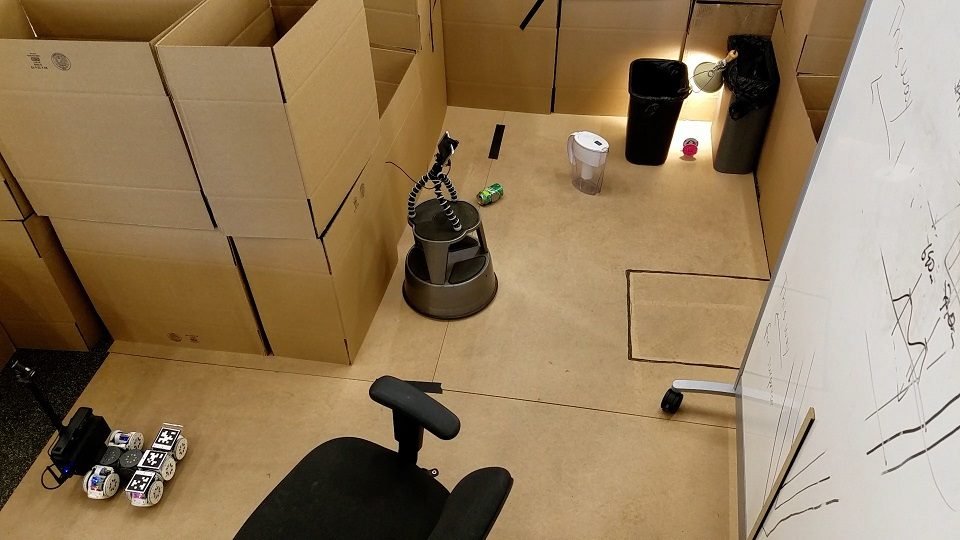
\includegraphics[width=\Lwidth]{images/overhead_starting.jpg}}
%
& \pbox{\Rwidth}{\textbf{Experiment I:} Explore environment to find all pink or green objects and blue dropoff zone. Deliver all objects to dropoff zone.}\\

 & \vspace{-5pt}\\
\hline
 & \vspace{-5pt}\\
 
\raisebox{\Rboxheight}{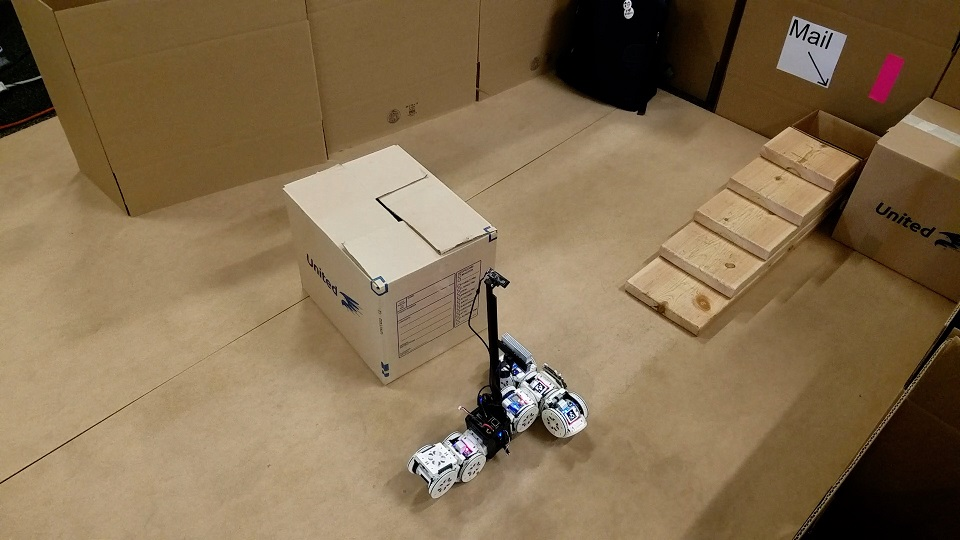
\includegraphics[width=\Lwidth]{images/stairs_explore_overhead.jpg}}
%
& \pbox{\Rwidth}{\textbf{Experiment II:} Explore environment to find mailbox, then deliver a circuit to the box.}\\

 & \vspace{-5pt}\\
\hline
 & \vspace{-5pt}\\
 
\raisebox{\Rboxheight}{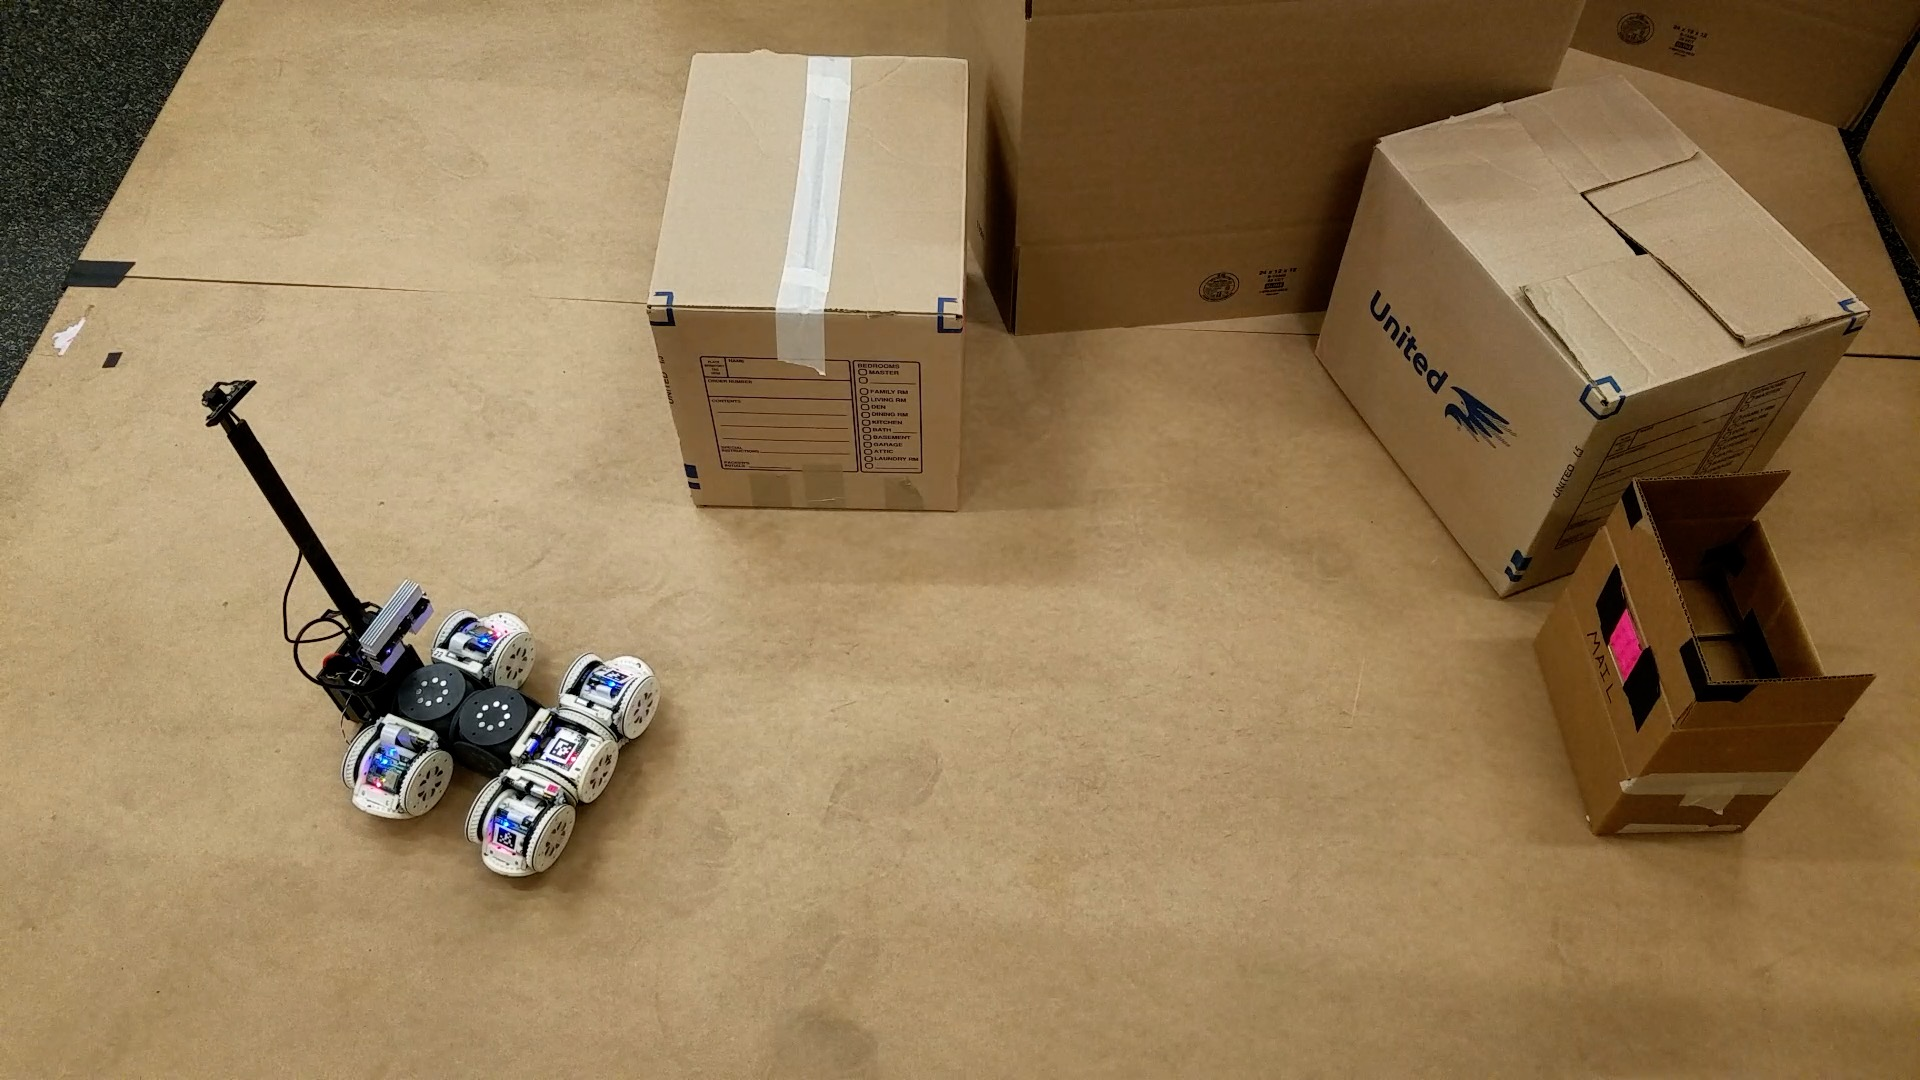
\includegraphics[width=\Lwidth]{images/stamp_explore_overhead.jpg}}
%
& \pbox{\Rwidth}{\textbf{Experiment III:} Explore environment to find package, then place a stamp on the package.}\\

 & \\
\hline
\end{tabular}
\caption{Environments and tasks for hardware experiments}
\label{table:task-compare}
\end{table}
\setlength{\tabcolsep}{6pt} % resetting to default

\subsection{Experiment I}
%
Experiment I tasks the robot with cleaning a messy graduate student office.  Figure \ref{fig:map} illustrates the environment layout. The robot must explore the unknown office environment and search for any green- or pink-colored metal garbage that can be recycled.  The robot must find, retrieve, and deliver all metal garbage to a designated drop-off zone for recycling, which is marked with a blue square on the wall.

The high-level task is compact, consisting of three sub-tasks: explore the environment, find and retrieve all metal objects, and deliver each to the drop-off zone.  Successful completion of the task in the given environment requires complex behavior that fully utilizes the robot's exploration, reconfiguration, and manipulation abilities. The environment contains two colored objects: a green soda can in the open (a ``free'' environment type), and a pink spool of wire in a narrow gap between two trash cans (a ``tunnel'' environment). Although the colors of the target objects are known \textit{a priori}, the types of environments surrounding the objects, the locations of the objects and drop-off zone, and obstacles in the environment are unknown \textit{a priori}.  Note that the object colors (pink and green) have no influence on environment characterization: in other words, the robot does not know that the pink object is in a ``tunnel''  before the experiment starts.  Both objects have small pieces of steel attached, giving the modules something to grasp using their magnetic connectors.

Five SMORES-EP modules, one Sensor Module\footnote{This experiment uses an older version of the sensor module.  The body is larger (160 $\times$ 80 $\times$ 80mm box), and it uses an older Asus Xtion Pro Live RGB-D camera, which is larger than the Orbecc Astra but provides similar data.  The only functional difference between this older sensor module and the version presented in Section~\ref{sec:sensor_module} is the larger size.}, and three passive cubes composed the robot for performing the task. 
During the experiment, the high-level planner used the library of configurations and behaviors described in Section \ref{sec:configuration-specifics}.

% Map
\begin{figure}
\begin{center}
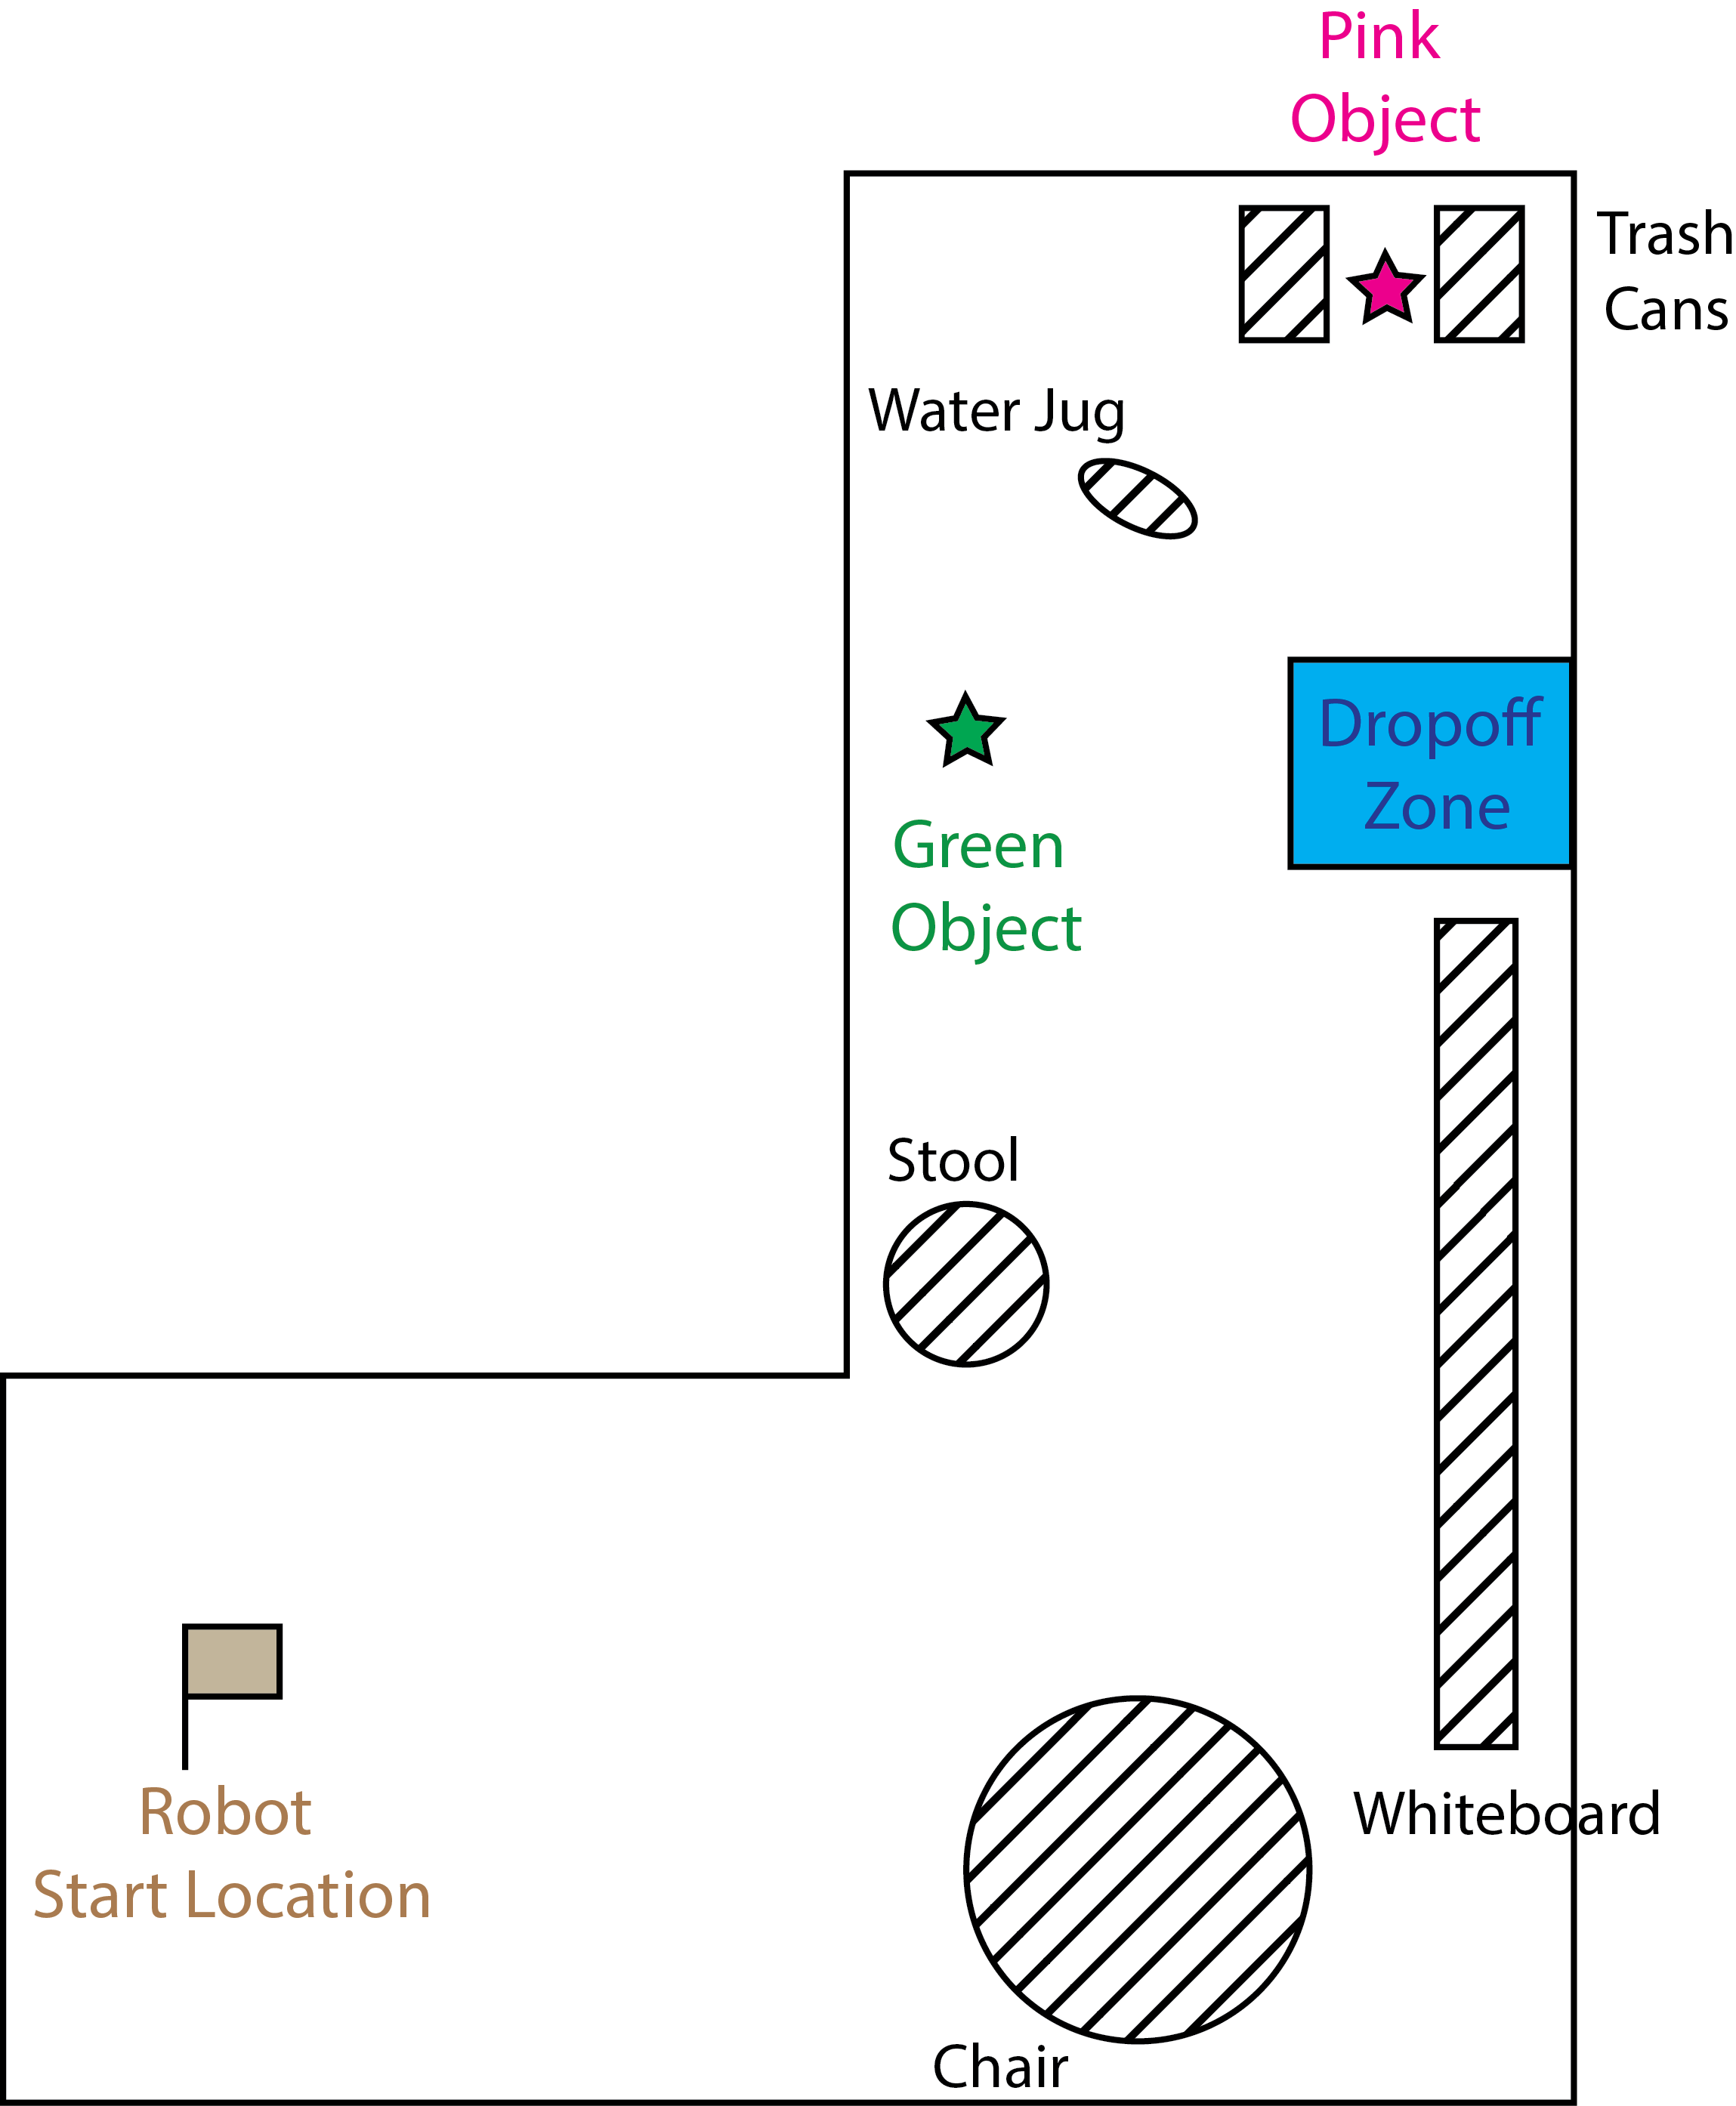
\includegraphics[width=0.3\textwidth]{images/RSSMap.png}
\caption{Diagram of Experiment I environment}
\vspace{-2em}
\label{fig:map}
\end{center}
\end{figure}

\begin{figure*}[t]
      \centering
      \begin{subfigure}[t]{0.32\textwidth}
        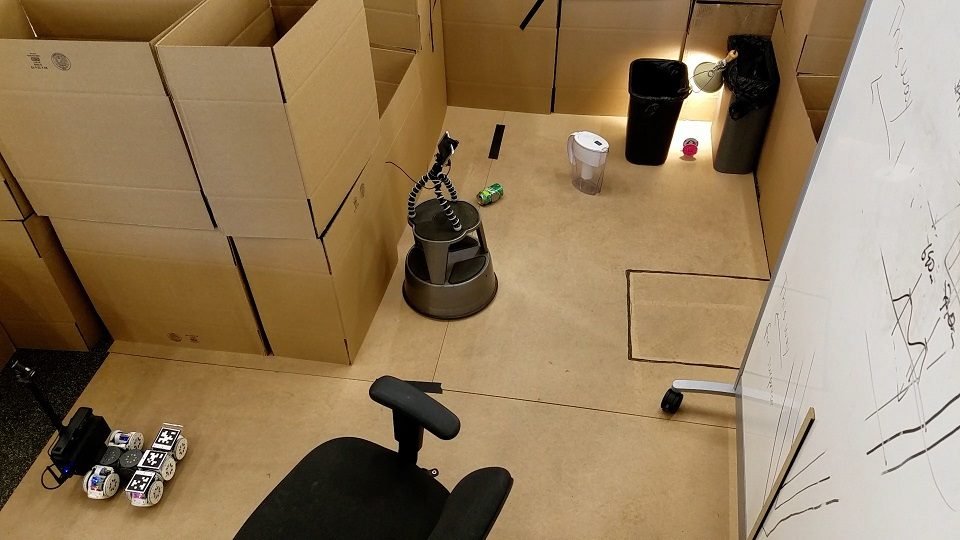
\includegraphics[width=\textwidth]{images/overhead_starting.jpg}
        %\label{fig:obja}
        \caption{Environment and robot starting location}
    \end{subfigure}
    \begin{subfigure}[t]{0.32\textwidth}
        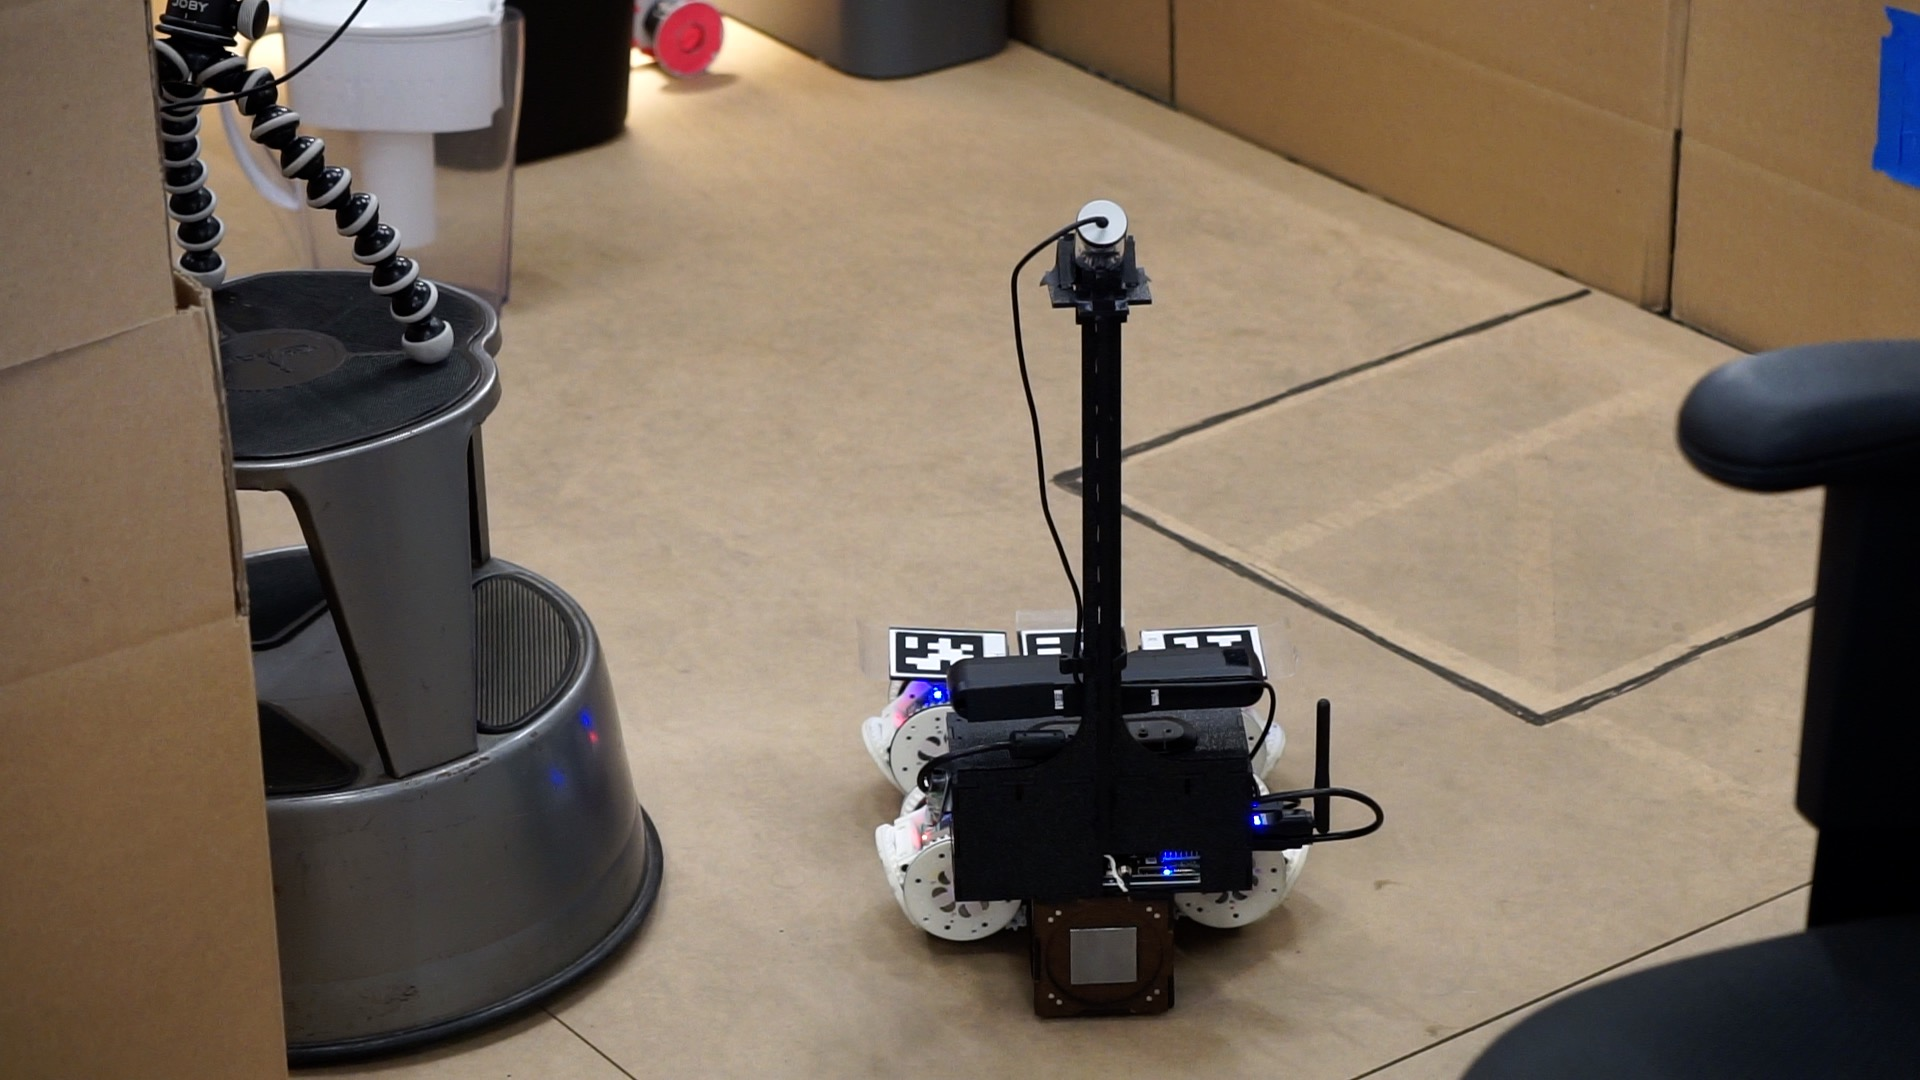
\includegraphics[width=\textwidth]{images/exploration.jpg}
        %\label{fig:objb}
        \caption{Exploring  while searching for objects}
    \end{subfigure}
    \begin{subfigure}[t]{0.32\textwidth}
        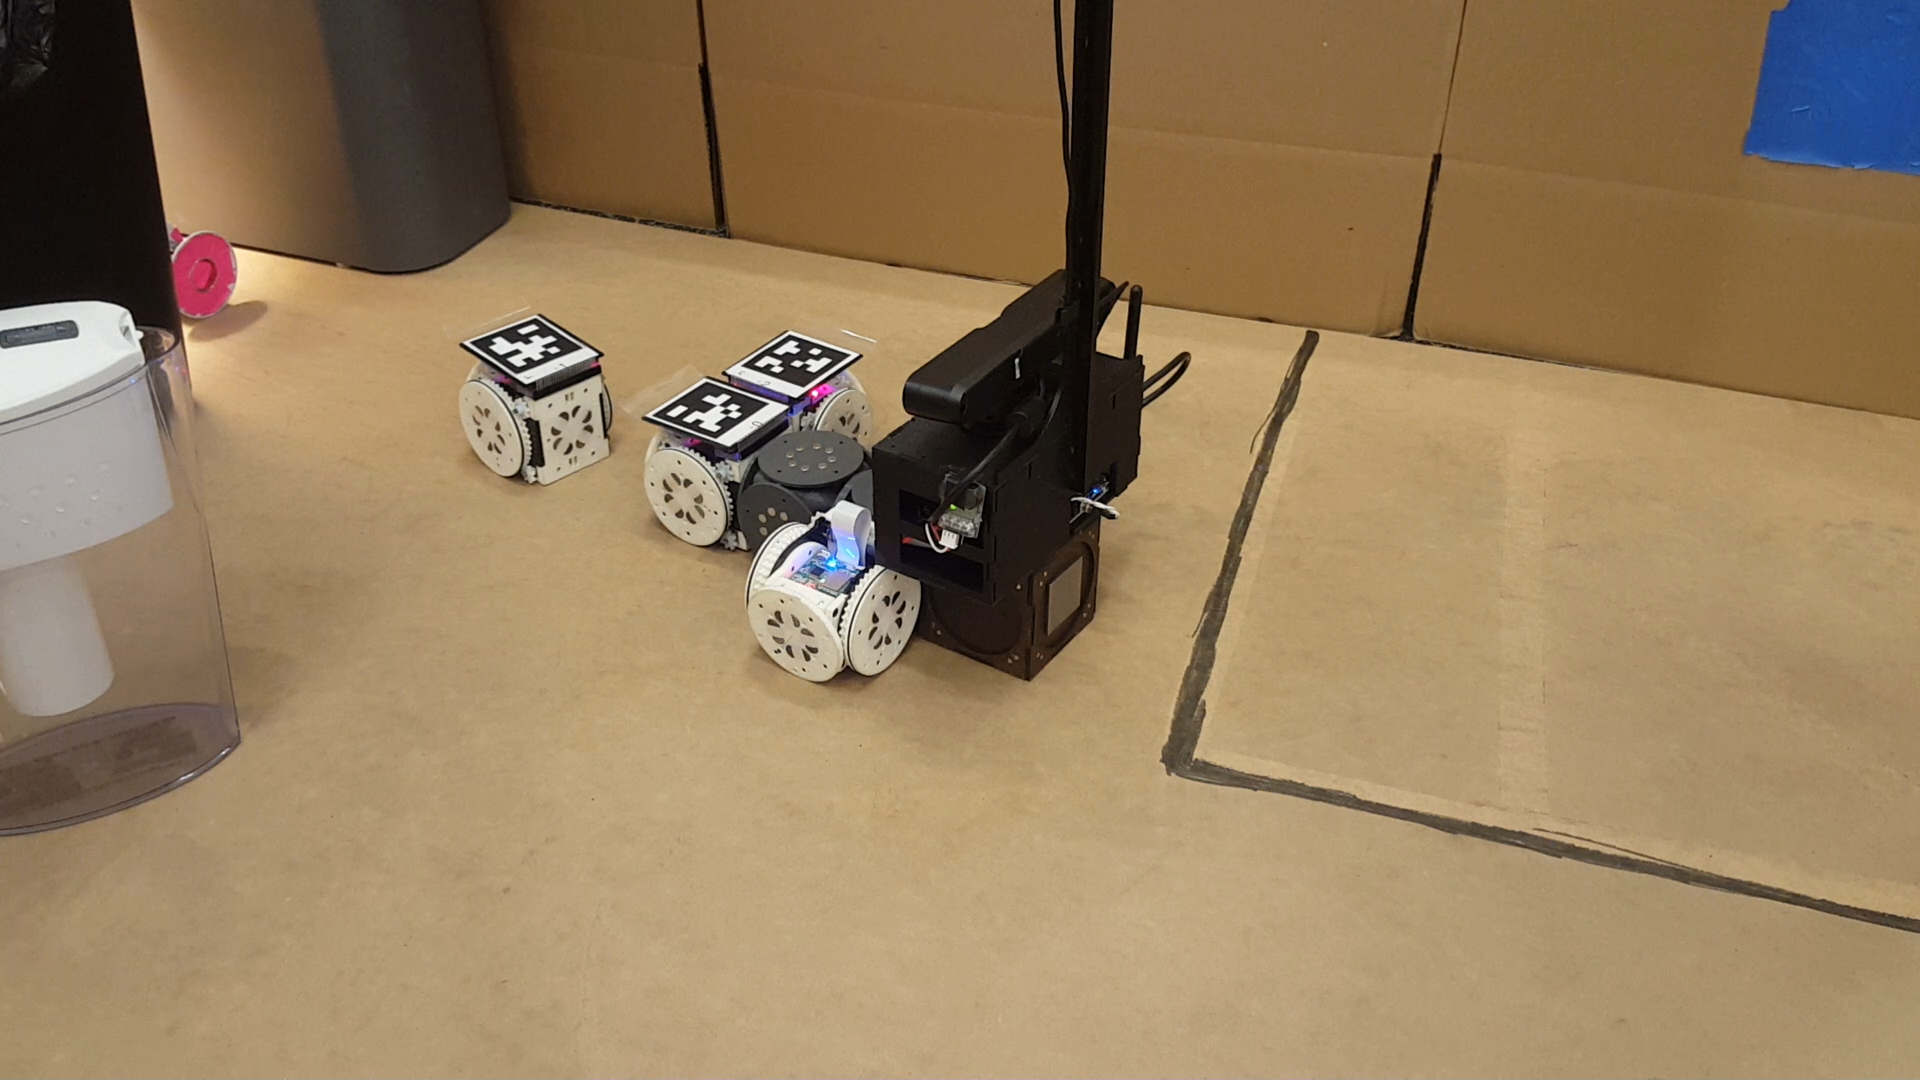
\includegraphics[width=\textwidth]{images/reconfiguration.png}
        %\label{fig:objb}
        \caption{Reconfiguring to retrieve pink object}
    \end{subfigure}
    \begin{subfigure}[t]{0.32\textwidth}
        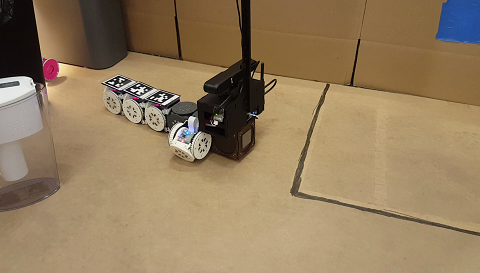
\includegraphics[width=\textwidth]{images/pink_retrieval.png}
        \caption{Retrieving pink object}
        \label{fig:pink_grab}
    \end{subfigure}
    \begin{subfigure}[t]{0.32\textwidth}
        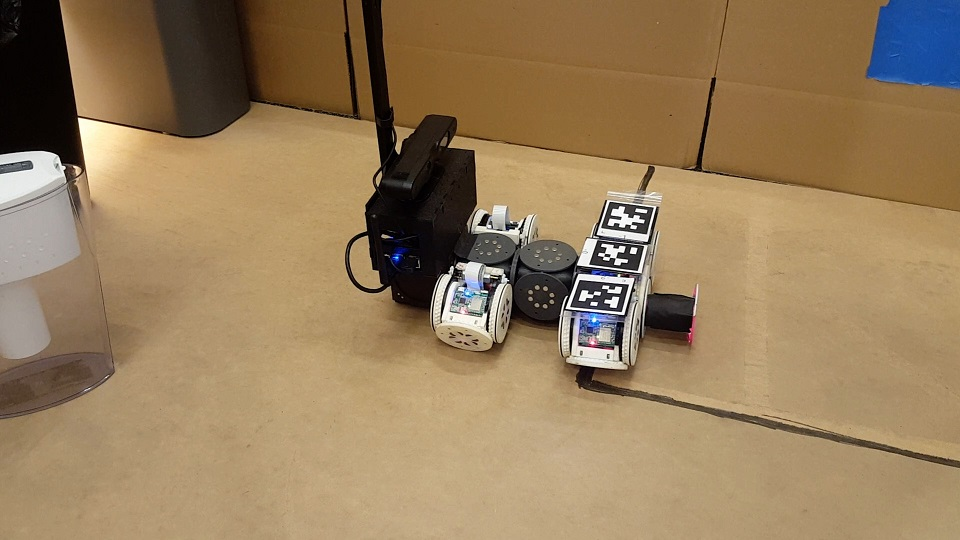
\includegraphics[width=\textwidth]{images/dropoff.jpg}
        \caption{Depositing an object in the drop-off zone}
        \label{fig:dropoff}
    \end{subfigure}
    \begin{subfigure}[t]{0.32\textwidth}
        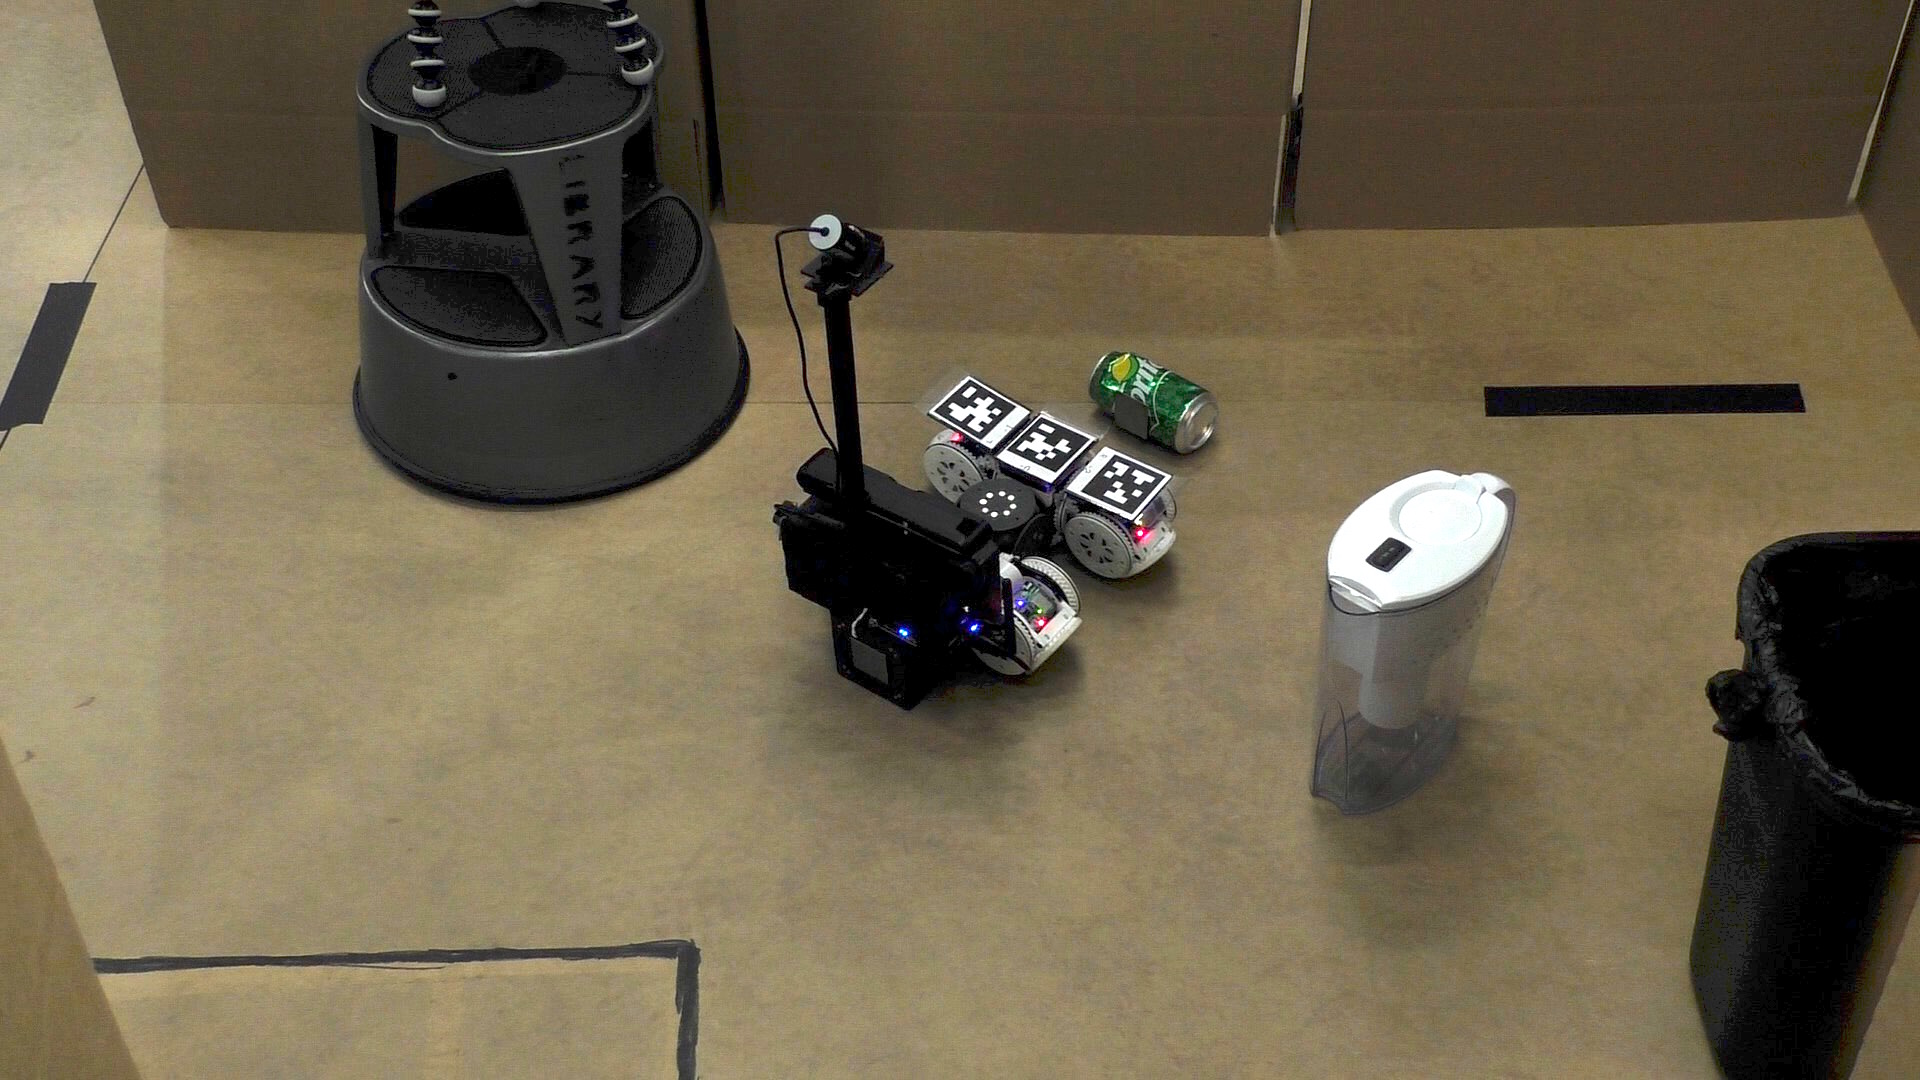
\includegraphics[width=\textwidth]{images/green_retrieval.jpg}
        %\label{fig:objb}
        \caption{Retrieving green object}
    \end{subfigure}
      \caption{Phases of Experiment I.}
      \label{fig:demo}
   \vspace{-1em}
   \end{figure*}
%
Figure \ref{fig:demo} shows snapshots from the experiment run. A video of the entire experiment is available as an attachment to this paper. The robot starts in the ``Car'' configuration. The starting location prevents the robot from seeing the objects initially, forcing it to explore the environment. After a period of exploration, the robot locates the pink object. The characterization algorithm correctly classifies the surrounding environment as a ``tunnel'' type, and gives this classification to the high-level planner. Based on this classification, the high-level planner directs the robot to navigate in front of the object and reconfigure to the ``Proboscis'' configuration. The ``Proboscis'' then uses its long arm to reach into the tunnel and pull the object out into the open.

 The ``Proboscis'' can only drive forwards and backwards (it cannot turn), so the robot concludes that it must reconfigure back to the ``Car'' to drive the object to the drop-off zone.  To do so, the robot drops the object, reconfigures, and picks the object back up. The ``Car'' then navigates to and drops off the object at the drop-off zone, which the robot previously located during exploration and recorded in the global map built by the SLAM algorithm.

After delivering the pink object, the robot navigates directly to the green object, discovered while dropping off the pink object. The robot correctly determines that the green object is in a ``free'' environment, and picks it up without reconfiguring. The robot finishes the experiment by also delivering the green object to the drop-off zone. Figure \ref{fig:octomap} shows a volumetric map of the environment generated as the robot explores and delivers objects. The robot successfully completed all tasks in the experiment in approximately 26 minutes.

Note that at one point in the video a person reaches onto the field to dislodge the green object from a crack in the floor.  This was due to a defect in the experimental setup (which is not supposed to have a crack in the floor) and not an error in the robot's performance.
%
\begin{figure}
\begin{center}
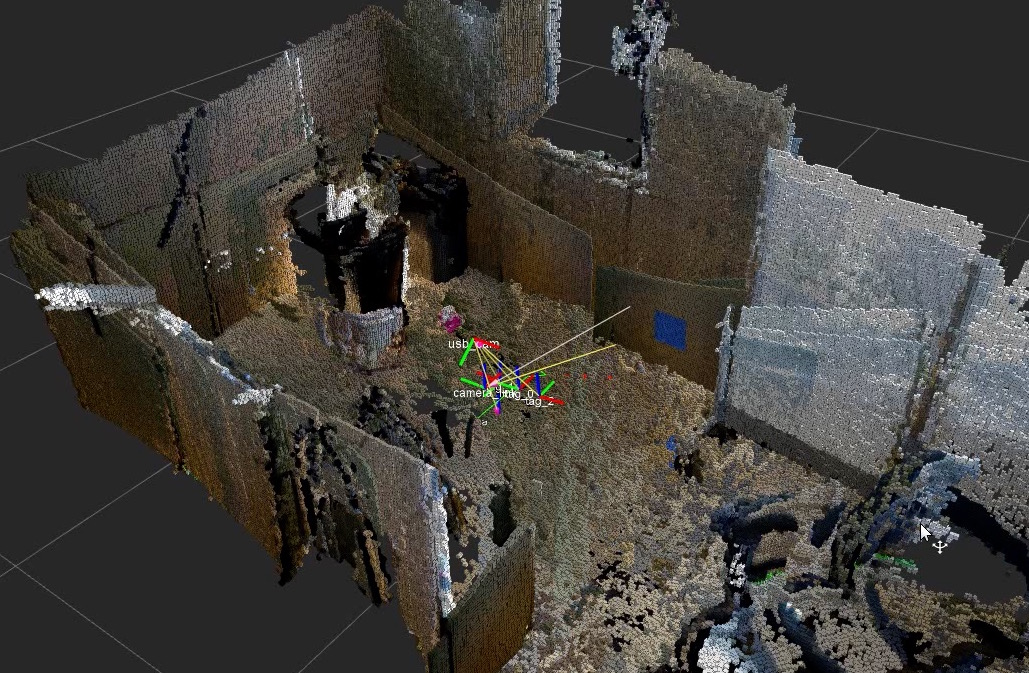
\includegraphics[width=0.4\textwidth]{images/map4.jpg}
\caption{Volumetric map of environment built by visual SLAM}
\vspace{-2em}
\label{fig:octomap}
\end{center}
\end{figure}

\subsection{Experiment II}
%
In Experiments II and III, the robot helps researchers at the University of Pennsylvania mail a circuit board to collaborators at Cornell.  First, in Experiment II, the robot must place the circuit board in a mailbox, and then in Experiment III, the robot must place a postage stamp on the box so that it can be shipped.  Experiments I and II have the same high-level task specification: starting with an object in its possession, the robot must explore until finding a drop-off point, then deposit the object at the drop-off point.

%%%%%%%%%%%%%%%

%The second and third experiments were designed to demonstrate the breadth of our system's adaptive capabilities. As such, these two experiments included the same high-level task specification that is different from the task in Experiment I. However, differing environments between Experiment II and Experiment III force the robot to adapt differently while performing the task.
%For Experiment II, the robot is given a circuit that needs to be shipped, and is tasked with finding the shipping bin in which to place the circuit.
%The high-level task includes sub-tasks of exploring the unknown environment, locating and characterizing the environment surrounding the mail bin, and delivering the package to the bin.

The environment setup for Experiment II (see Table \ref{table:task-compare}) includes an obstacle (cardboard box), a staircase, and the mailbox at the top of the staircase.  A pink rectangle indicates the mailbox.  Note that this scenario is identical to the mail delivery example mentioned as motivation earlier in the paper.

%The full performance of the experiment is included in the video attachment to this paper.
The robot begins the experiment in the ``Scorpion'' configuration with its view of the staircase and mailbox blocked by the cardboard box.  After a short period of exploration, the robot observes and recognizes the mailbox, and characterizes the surrounding environment as ``stairs''. Based on this characterization, the high-level planner directs the robot to use the ``Snake'' configuration to traverse the stairs. Using the 3D map and characterization of the environment surrounding the mail bin, the robot navigates to a point directly in front of the stairs, faces the bin, and reconfigures to the ``Snake'' configuration. The robot then executes the stair climbing gait to reach the mail bin, and drops the circuit successfully. It then descends the stairs and reconfigures back to the ``Scorpion'' configuration to end the mission.

\begin{figure}[t]
      \centering
      \begin{subfigure}[t]{0.24\textwidth}
        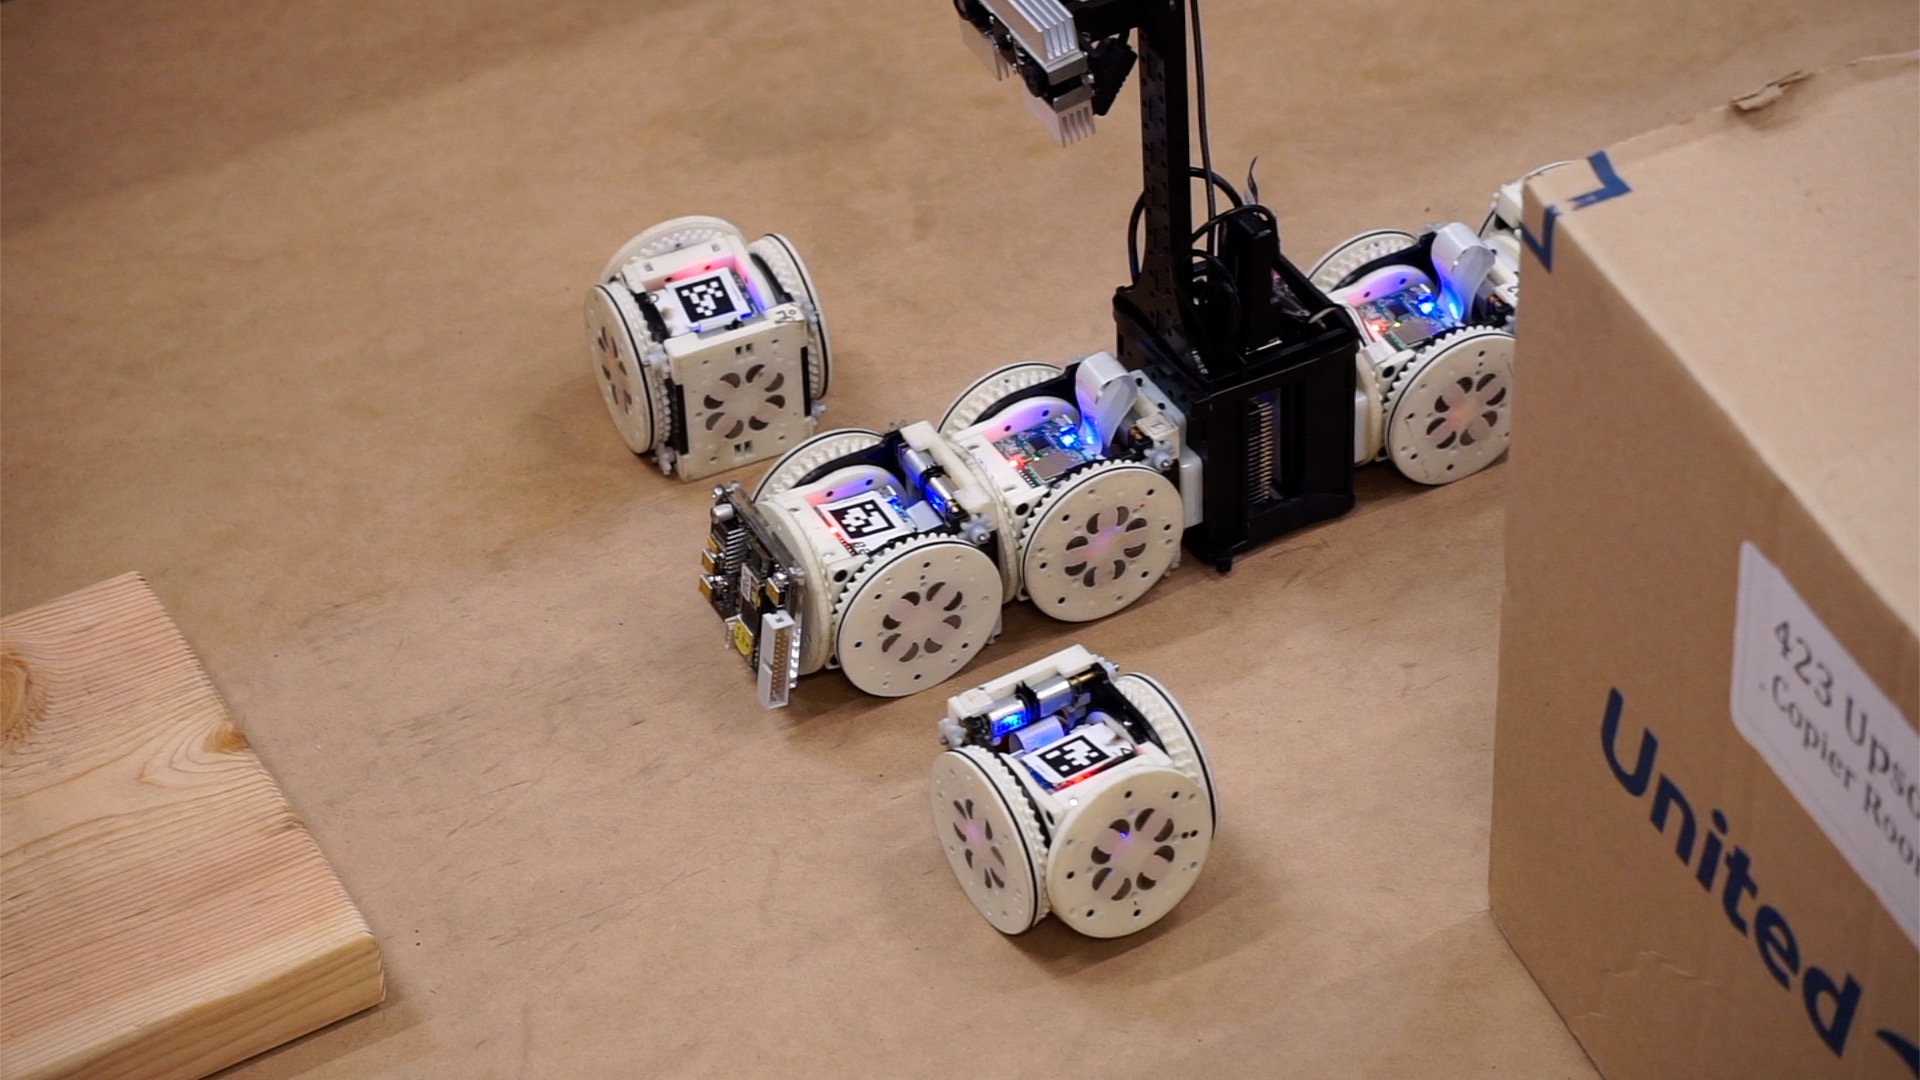
\includegraphics[width=\textwidth]{images/stairs_reconfig.jpg}
        %\label{fig:obja}
        \caption{Reconfiguring to climb stairs}
    \end{subfigure}
    \begin{subfigure}[t]{0.24\textwidth}
        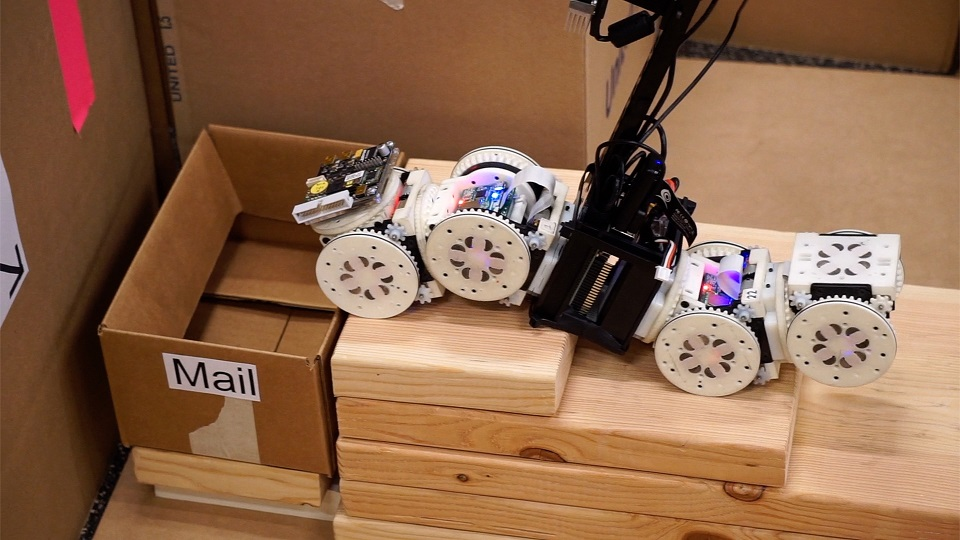
\includegraphics[width=\textwidth]{images/stairs_climb.jpg}
        %\label{fig:objb}
        \caption{Successful circuit delivery}
    \end{subfigure}
    
    \begin{subfigure}[t]{0.24\textwidth}
        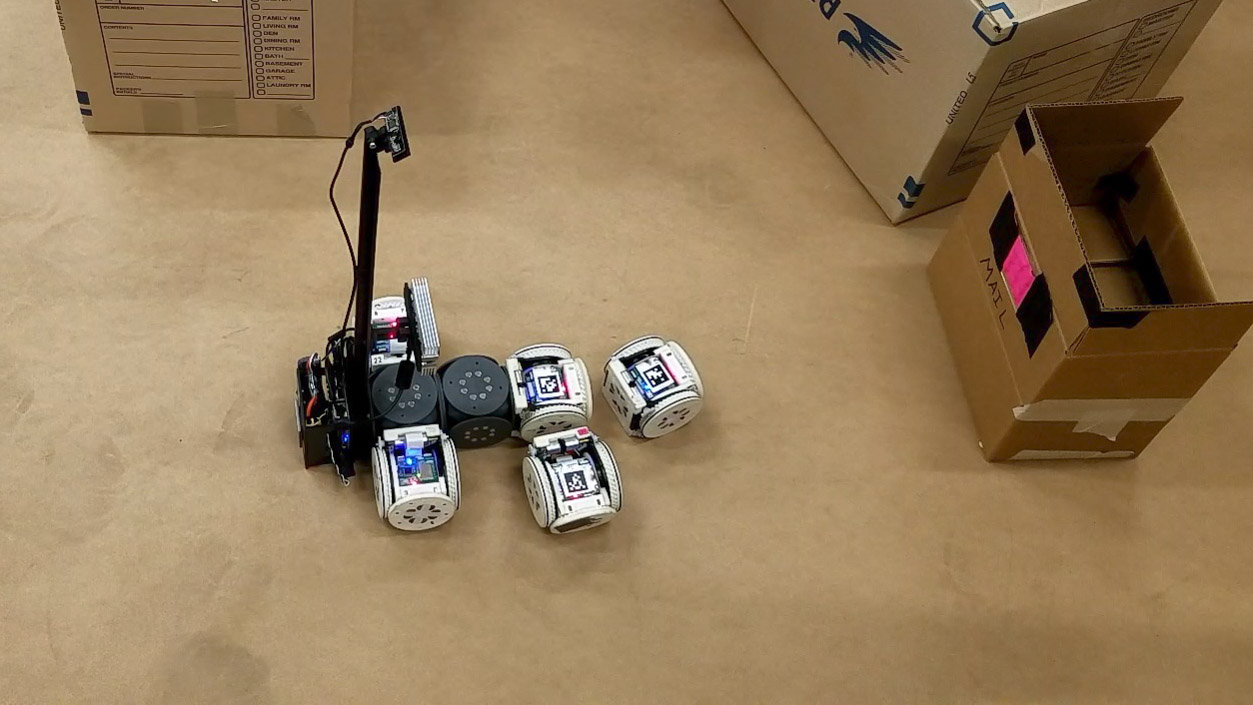
\includegraphics[width=\textwidth]{images/stamp_reconfig.jpg}
        %\label{fig:objb}
        \caption{Reconfiguring to place stamp}
    \end{subfigure}
    \begin{subfigure}[t]{0.24\textwidth}
        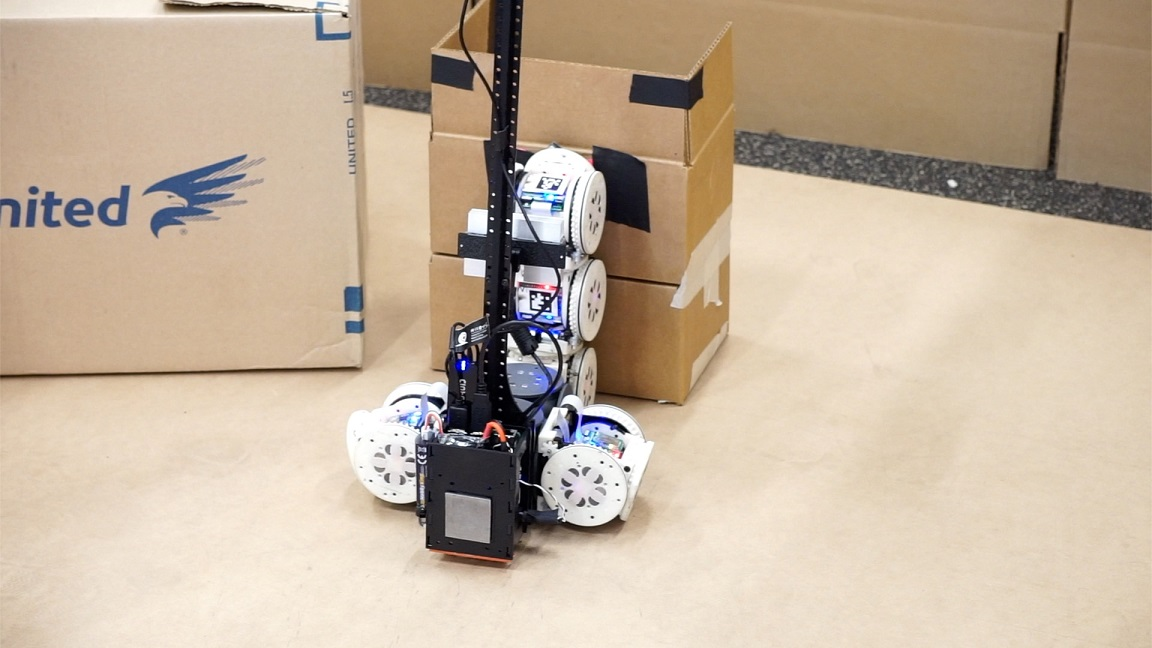
\includegraphics[width=\textwidth]{images/stamp_placing.jpg}
        %\label{fig:objb}
        \caption{Successful stamp placement}
    \end{subfigure}
      \caption{Experiments II and III.}
      \label{fig:exps}
   \end{figure}

\subsection{Experiment III}

For the final experiment, a student gives the robot a postage stamp\footnote{The postage stamp has a thin steel backing, so that the robot can pick it up with its magnets, and so that it adheres to magnets on the package.} to place on the package so that it can be shipped to Cornell. The high-level task has the same specification as in Experiment II: explore the unknown environment, find the delivery goal indicated by a pink area, and place the object at the target. The environment is different, most significantly in that the delivery goal is in a ``high'' environment type instead of the ``stairs'' environment used in Experiment II (see Table \ref{table:task-compare}).

%Please see the video attachment for the full performance of this experiment.
The robot begins in the ``Car'' configuration, and cannot see the package from its starting location.  After a short exploration, the robot identifies the pink square marking the package.  The pink square is unobstructed, but is approximately 25cm above the ground; the system correctly characterizes this as the ``high''-type environment, and recognizes that reconfiguration will be needed to reach up and place the stamp on the target.  The robot navigates to a position directly in front of the package, reconfigures to the ``Proboscis'' configuration, and executes the ``highReach'' behavior to place the stamp on the target, completing its task.
%
%     ____  _                           _
%    / __ \(_)___________  ____________(_)___  ____
%   / / / / / ___/ ___/ / / / ___/ ___/ / __ \/ __ \
%  / /_/ / (__  ) /__/ /_/ (__  |__  ) / /_/ / / / /
% /_____/_/____/\___/\__,_/____/____/_/\____/_/ /_/
\section{Discussion}
\label{sec:discussion}
The real-world experiments demonstrate that our system has the ability to autonomously reconfigure in response to observations in the environment in order to perform high-level tasks. The system performs complex tasks, determining robot actions and reconfiguration online in response to observations of the environment. The same system successfully performs two different high-level tasks. Experiments II and III demonstrate that the same high-level task can be performed in different environments, because the robot autonomously adapts to the challenges presented by each environment. Our system is the first to successfully demonstrate this level of perception-informed reconfiguration and autonomy.

In addition to demonstrating our system's abilities, the experiments revealed several insights related to perception-informed autonomy on MSRR systems. As this is the first successful system of its kind, we encountered many challenges with achieving robust performance, and discovered many limitations of the system implementation and with the modular robot hardware. We hope to share these observations to aid those who may wish to implement our system or improve its robustness and capability.
%
\subsection{Single-Sensor Architecture Enables Autonomy}
%
Autonomy in unknown environments requires powerful sensing capabilities.  Our centralized sensing architecture allowed the robot to carry a single, powerful RGB-D camera, enabling sophisticated capabilities like Visual SLAM and environment characterization. In contrast, previous systems that used distributed sensing have been forced to rely on less sophisticated sensors that can be carried by each module in the cluster, limiting their ability to operate autonomously in unknown environments.   Our system has demonstrated more sensor-based autonomy than any previous modular robot, and we believe this is due in large part to our decision to use a single, powerful sensor module.

Likewise, high-fidelity centralized sensing during reconfiguration, provided by AprilTags, allowed our implementation to transform between configurations quickly and reliably.  Each reconfiguration action (a module disconnecting, moving, and reattaching) takes about one minute, and succeeds about 85\% of the time.  In contrast, past systems required 5-15 minutes for single reconfiguration actions \cite{Yim2007, Rubenstein2004,Murata2006}, which would make it difficult to use them for the kinds of tasks we have demonstrated.

Centralized sensing has some drawbacks.  The sensor module is larger than a single SMORES-EP module, and is only compatible with configurations that can hold it in a good view of the robot's surroundings.  This also limits the kinds of behaviors that can be performed, because care must be taken to hold the sensor level and steady.  The configurations and behaviors used in our experiments move more slowly than in past experiments with SMORES-EP, in part for this reason. Supporting the sensor module while traversing obstacles and rough terrain is particularly challenging.  In Experiment II, we used rigid connectors to attach the sensor module to the surrounding SMORES-EP modules, in order to avoid connection breakage when climbing the stairs. 

Centralized sensing also limits reconfiguration. Since modules can only move in 2D within the camera view,  some reconfigurations are not possible.  For example,  the ``Car'' cannot reconfigure into the ``Snake'' using  our implementation, because the camera cannot see the back wheels of the ``Car''. Consequently, if the robot had started out as the ``Car'' at the beginning of Task 3, it would not have been able to complete its task.

We believe the benefits provided to our system by centralized sensing outweigh the costs.  The decision represents a tradeoff, sacrificing some of the flexibility of the modular system to achieve more capability and autonomy.  As future modular systems move out of the lab and into real-world deployment, it will become increasingly important for designers to consider similar tradeoffs.

It's worth noting that while our implementation relies in part on external computation and wireless network access, this is not a fundamental system requirement.   In fact,  in our implementation the majority of  heavy computation (mapping, navigation, video processing) was done onboard on the sensor module, with a few processes (high-level planner, reconfiguration planner, and next-best-view planner) run offboard, primarily for development convenience. % 
In the future we believe everything could be run onboard with only minor adjustments.
%
\subsection{Strengths - Reactive Capability}
%
%{\color{red}(Specifying high-level tasks:)}
The high-level planner, environment characterization tools, and library work together to allow tasks to be represented in a flexible and reactive manner. For example, at the high level, Experiments II and III are the same task: deliver an object at a point of interest.  However, after characterizing the environment, the system determines that vastly different behaviors are required to complete the task, and in both cases, that reconfiguration is needed before the appropriate behavior can be performed. Similarly, in Experiment I there is no high-level distinction between the green and pink objects - the robot is simply asked to retrieve all objects it finds.  The sensed environment once again dictates the choice of behavior: the simple problem is solved in a simple way (green object), and the more difficult problem is solved in a more sophisticated way (pink object).

%{\color{red}(Interacting:)}
We selected the three scenarios in our experiments to showcase a range of different ways SMORES-EP can interact with environments and objects: movement over flat ground, fitting into tight spaces, reaching up high, and climbing over rough terrain, and manipulating objects.  This broad range of functionality is impressive for such a small robot, and is only accessible to SMORES-EP by reconfiguring between different morphologies.
%
\subsection{Major Challenge - Robustness}
%
\begin{table}
\centering
\begin{tabular}{|c|c|c|}
\hline
\textbf{Reason of failure} & \textbf{Number of times} & \textbf{Percentage}\\ 
\hline
Hardware Issues & 10 & 41.7\% \\ 
\hline
Navigation Failure & 3 & 12.5\% \\ 
\hline
Perception-Related Errors & 6 & 25\% \\ 
\hline
Network Issues & 1 & 4.2\% \\ 
\hline
Human Error & 4 & 16.7\% \\ 
\hline
\end{tabular}
\caption{Reasons for experiment failure.}
\label{table:errors}
\end{table}
%
Our implementation is vulnerable to small errors - if things go wrong in the course of completing a task, the entire task will likely fail. 
Table \ref{table:errors} shows the causes of failure for 24 attempts of Experiment II (placing the stamp on the package).  
Nearly all failures are due to an error in one of the low-level components the system relies on.
42\% of failures were due to hardware errors, and 38\% were due to failures in low-level software (object recognition, navigation, environment characterization). 
These components were designed for research, not real-world deployment, and could be engineered to perform much more reliably in a production setting.

The simulator served as a valuable prototyping tool, but all behaviors required significant
fine-tuning in hardware before they would run reliably.  
Open-loop behaviors like stair-climbing and reaching up to place the stamp are fairly
inflexible with respect to environment conditions, and also vulnerable to hardware
errors like poorly calibrated encoders.  
Behaviors like exploration and reconfiguration use the sensor module to close the
loop, and are significantly less vulnerable to these kinds of errors.  
However, these behaviors required much more up-front development effort.

Lack of robustness is  a weakness of the system architecture.  The high-level planner assumes all underlying components are reliable and robust, so if any low-level component fails, the high-level planner might behave unexpected and the entire task may fail. In the future, we will explore high-level strategies for error recovery: for example, recognizing that a module has failed and adapting the approach so that task will not fail entirely.
%
\subsection{Challenges for Future Systems}
%
Based on our small-scale, proof of concept experiments, we believe this system has the potential to be scaled and deployed in a real-world setting. Our experiences have provided us with some insight into the challenges future systems might face.

%{(\color{red} Gathering information:)}
We opted to use simple techniques for navigation, object recognition, and differentiating between environments, which were suitable for our proof-of-concept experiments. To deploy a similar system in real life, more sophisticated techniques would be needed. Considering the ongoing trend towards high-performance sensors and computers at small sizes, we would expect that implementing these sophisticated techniques onboard the sensor module will become easier over time.

%{\color{red}(Moving around:)}
The ability of the robot to move and maneuver in the environment relies heavily on the hardware.  The SMORES-EP designs we used for exploration move slowly, and can only drive over smooth, flat ground.  In a demanding real-world application like search-and-rescue, the hardware system would likely need to be able to move more quickly.  In general, real-world application would require modules with more powerful actuators, and the ability to hold large payloads without breaking inter-module connections.

In theory, the system architecture places no fundamental limitations on the kinds of gaits or behaviors used to locomote in the environment.  However, our architecture does require a suitable \textit{motion model} and \textit{path planner} for any behavior used for locomotion.  In practice, this means that while a modular robot may be capable of a large number of creative or unusual gaits for locomotion, those that conform to standard, well-understood motion models (like differential or holonomic drive) require much less effort to implement, and often end up being the most useful for actually accomplishing tasks.

%In general, the range of ways in which the robot may interact with its environment is determined by the contents of the design library, which would ideally contain a large number of configurations and behaviors suitable for a diverse set of tasks.
The fact that our architecture relies upon a discrete representation of behaviors could mean that a real-world implementation would require a very large library, which presents some challenges. To precisely describe capabilities and limits of each behavior, the system would need a large set of attributes when labeling library entries. As a result, users will need to understand all these attributes and use accurate ones when specifying the robot tasks. 
When searching the library for behaviors with user specified constraints, our method scales linearly with respect to the size of the library.%, which makes the system suitable in real-world experiments.

It is important to consider how the presented system could be adapted to work with
other modular robot hardware. Our system relies on a 3D sensor for performing RGB-D
SLAM, sufficient onboard processing power for perception and control algorithms,
and a robust modular hardware system with a versatile self-reconfiguration ability
that doesn't rely on external sensors. As long as another MSRR system provides these
features and its own hardware-specific and reconfiguration controllers, our system
can be integrated into it for performing high-level tasks.
%
\subsection{Conclusion}
%
To conclude, this paper presents the first MSRR system that uses perception of an unknown environment to reactively perform complex high-level tasks using intelligent reconfiguration. Components of this system include novel controller synthesis, environment characterization, and self-reconfiguration methods. The demonstration of this novel capability is crucial to the success of modular robots as a technology, and takes a step toward the application of modular robots to tasks in the real world.
%
%\section*{Acknowledgments}
%
%This work was funded by NSF grant numbers CNS-1329620 and CNS-1329692.


       %     ____       ____
       %    / __ \___  / __/__  ________  ____  ________  _____
       %   / /_/ / _ \/ /_/ _ \/ ___/ _ \/ __ \/ ___/ _ \/ ___/
       %  / _, _/  __/ __/  __/ /  /  __/ / / / /__/  __(__  )
       % /_/ |_|\___/_/  \___/_/   \___/_/ /_/\___/\___/____/

%% Use plainnat to work nicely with natbib. 
\bibliographystyle{IEEEtran}
\bibliography{references}


\begin{IEEEbiography}
    [{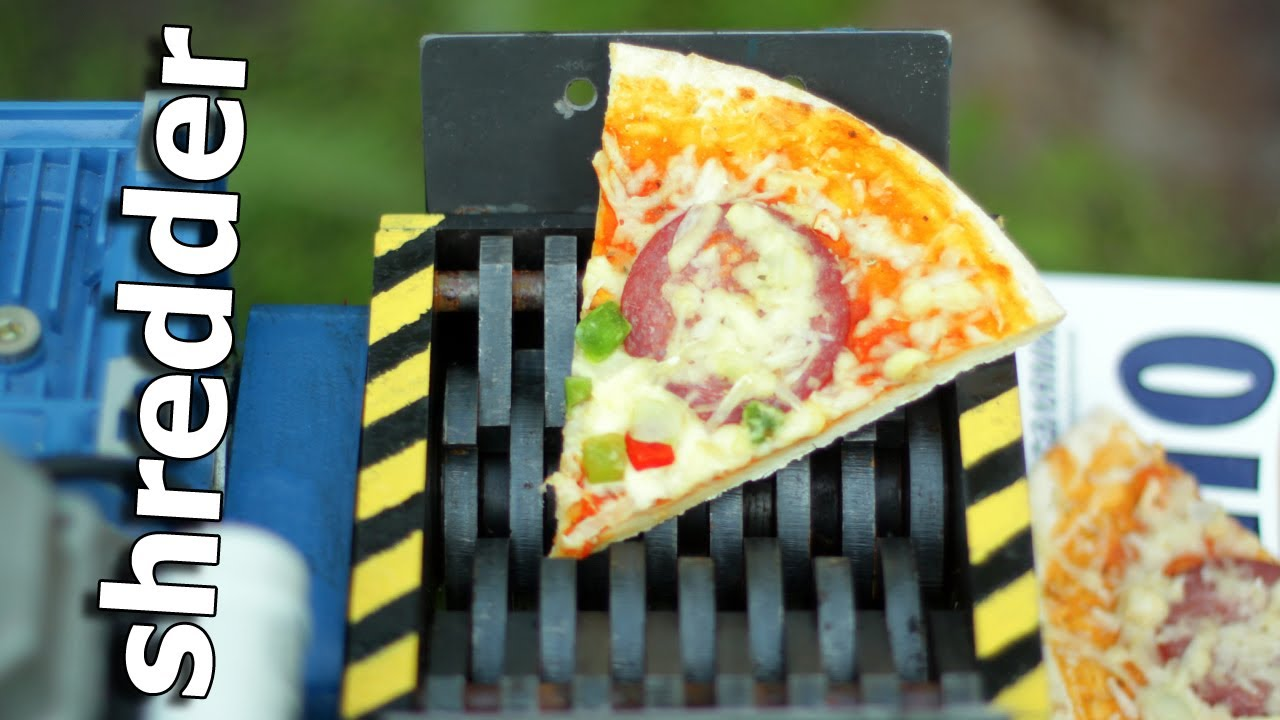
\includegraphics[width=1in,height=1.25in,clip,keepaspectratio]{images/jonathan.jpg}}]{Jonathan Daudelin a.k.a The Pizza Shredder}
He shreds pizza...
\end{IEEEbiography}

% if you will not have a photo at all:
\begin{IEEEbiographynophoto}{Gangyuan Jing}
is currently a Ph.D candidate in the Verifiable Robotics Research Group at Cornell University. His research focuses on synthesizing controllers from high-level robot tasks with modular robot systems, and improving the optimality of the correct-by-construction controllers. He received the Best Systems Paper Award at RSS 2016, in addition to being a finalist for the Best Paper and the Best Student Paper awards.
\end{IEEEbiographynophoto}

% insert where needed to balance the two columns on the last page with
% biographies
%\newpage

\begin{IEEEbiographynophoto}{Tarik Tosun}
received the B.S.E. degree in Mechanical and Aerospace Engineering from Princeton University, Princeton, NJ, USA in 2012. Currently, he is working towards the Ph.D. degree at the University of Pennsylvania, Philadelphia, PA, USA in the Modlab, a part of the GRASP Laboratory. His interests include modular robots, and automatic synthesis of robot designs from task requirements. Mr. Tosun is a National Science Foundation Graduate Research Fellow and a member of Tau Beta Pi. He received the Best Systems Paper Award at RSS 2016, in addition to being a finalist for the Best Paper and the Best Student Paper awards.
\end{IEEEbiographynophoto}

\begin{IEEEbiographynophoto}{Mark Yim}
is a Professor in the Mechanical Engineering and Applied Mechanics Department at the University of Pennsylvania.  Prior to Penn, he was Principal Scientist at the Palo Alto Research Center (formerly Xerox PARC).  His group designs and builds small flying robots, self-assembling structures, and modular self-reconfigurable robots, and has demonstrated robots that can transform into different shapes, jump, climb, manipulate objects and reassemble themselves.  Recently, his work has followed a theme of simplicity and low cost.  His other research interests include product design, reactive art and architecture, origami, snake locomotion, urban search and rescue and mobile manipulation.  Honors include the Lindback Award for Distinguished Teaching (UPenn's highest teaching honor); induction as a World Technology Network Fellow; and induction to MIT's TR100 in 1999.  He has over 200 publications and patents issued (perhaps most prominent are related to the video game vibration control which resulted in over US\$100 million in litigation and settlements) and has started two companies. He received the Best Systems Paper Award at RSS 2016, in addition to being a finalist for the Best Paper and the Best Student Paper awards.
\end{IEEEbiographynophoto}

\begin{IEEEbiographynophoto}{Hadas Kress-Gazit}
received her Ph.D. in Electrical and Systems Engineering from the University of Pennsylvania in 2008. She is currently an Associate Professor at the Sibley School of Mechanical and Aerospace Engineering at Cornell University. Her research focuses on creating verifiable robot controllers for complex high-level tasks using logic, verification methods, synthesis, hybrid systems theory and computational linguistics. She is a recipient of the NSF CAREER award in 2010 and was a finalist for the Best Student Paper Award at ICRA 2007 and a finalist for the Best Paper award at IROS 2007. She received the Best Systems Paper Award at RSS 2016, in addition to being a finalist for the Best Paper and the Best Student Paper awards.
\end{IEEEbiographynophoto}


\end{document}
